\chapter{%
    Tabular and Latent Space Synthetic Data Generation: A Literature Review
}~\label{chp:synthetic-data-review}
\graphicspath{{figures/synthetic-data-review/}}

\begin{adjustwidth}{30pt}{30pt}

    The generation of synthetic data can be used for anonymization,
    regularization, oversampling, semi-supervised learning, self-supervised
    learning, and several other tasks. Such broad potential motivated the
    development of new algorithms, specialized in data generation for specific
    data formats and Machine Learning (ML) tasks. However, one of the most
    common data formats used in industrial applications, tabular data, is
    generally overlooked; Literature analyses are scarce, state-of-the-art
    methods are spread across domains or ML tasks and there is little to no
    distinction among the main types of mechanism underlying synthetic data
    generation algorithms. In this paper, we analyze tabular and latent space
    synthetic data generation algorithms. Specifically, we propose a unified
    taxonomy as an extension and generalization of previous taxonomies, review
    70 generation algorithms across six ML problems, distinguish the main
    generation mechanisms identified into six categories, describe each type
    of generation mechanism, discuss metrics to evaluate the quality of
    synthetic data and provide recommendations for future research. We expect
    this study to assist researchers and practitioners identify relevant gaps
    in the literature and design better and more informed practices with
    synthetic data.

\end{adjustwidth}

\vspace{.5cm}
\textbf{Keywords:} Synthetic Data; Data Augmentation; Oversampling;
Regularization; Privacy

\section{Introduction}\label{sec:introduction}


Tabular data consists of a database structured in tabular form, composed of
columns (features) and rows (observations)~\cite{yoon2020vime}. It is one of
the most commonly used data structures within a wide range of domains.
However, ML techniques developed for tabular data can be applied to any type
of data; input data, regardless of its original format, can be mapped into a
manifold, lower-dimensional abstraction of the input data and mapped back into
its original input space~\cite{kingma2019introduction, DeVries2017}.
This abstraction is often referred to as embeddings, encodings, feature
space, or latent space. In this paper, we will refer to this concept as
latent space.

Synthetic data is obtained from a generative process based on properties of
real data~\cite{assefa2020generating}. The generation of synthetic data is
essential for several objectives. For example, it is used as a form of
regularizing ML classifiers (\textit{i.e.}, data
augmentation)~\cite{wang2021regularizing}. One form of anonymizing datasets is
via the production of synthetic observations (\textit{i.e.}, synthetic data
generation)~\cite{patki2016synthetic}. In settings where only a small portion
of training data is labeled, some techniques generate artificial data using
both labeled and unlabeled data with a modified loss function to train neural
networks (\textit{i.e.}, semi-supervised learning)~\cite{laine2017temporal}.
In imbalanced learning contexts, synthetic data can be used to balance the
target classes' frequencies and reinforce the learning of minority classes
(\textit{i.e.}, oversampling)~\cite{Fonseca2021}. Some active
learning frameworks use synthetic data to improve data selection and
classifier training~\cite{Kim2021}. Other techniques employ data
generation to train neural networks without labeled data (\textit{i.e.},
self-supervised learning)~\cite{grill2020bootstrap}.

The breadth of these techniques spans multiple domains, such as facial
recognition~\cite{lv2017data}, Land Use/Land Cover
mapping~\cite{Douzas2019rs}, medical image
processing~\cite{yi2019generative}, Natural Language Processing
(NLP)~\cite{feng2021survey} or credit card default
prediction~\cite{alam2020investigation}. Finding appropriate data
generation techniques varies according to the domain and data type. In
addition, several synthetic data generation methods are specific to the
domain, data type, or target ML task. Generally, these methods rely on
the domain data's structure and are not easily transferable to tabular
data.

Overall, synthetic data generation techniques for tabular data are not as
explored as image or text data, despite their popularity and
ubiquity~\cite{fakoor2020fast}. Furthermore, these techniques are invariant to
the original data format; they can be applied to both the latent
space~\cite{DeVries2017} or tabular data. On one hand, data generation
in the latent space uses a generative model to learn a manifold,
lower-dimensional abstraction over the input
space~\cite{kingma2019introduction}. At
this level, any tabular data generation mechanism can be applied and
reconstructed into the input space if necessary. On the other hand, synthetic
data generation on tabular data can be applied to most problems. Although, the
choice of generation mechanism depends on (1) the importance of the original
statistical information and the relationships among features, (2) the target
ML task, and (3) the role synthetic data plays in the process (\textit{i.e.},
anonymization, regularization, class balancing, etc.).  For example, when
generating data to address an imbalanced learning problem (\textit{i.e.},
oversampling), the relationships between the different features are not
necessarily kept, since the goal is to reinforce the learning of the minority
class by redefining an ML classifier's decision boundaries. If the goal is to
anonymize a dataset, perform some type of descriptive task, or ensure
consistent model interpretability, statistical information must be preserved.

Depending on the context, evaluating the quality of the generated data is a
complex task. For example, for image and time series data, perceptually small
changes in the original data can lead to large changes in the Euclidean
distance~\cite{assefa2020generating, theis2016note}. The evaluation of
generative models typically accounts primarily for the performance in a
specific task, since good performance in one criterion does not imply good
performance on another~\cite{theis2016note}. However, in computationally
intensive tasks it is often impracticable to search for the optimal
configurations of generative models. To address this limitation, other
evaluation methods have been proposed to assist in this evaluation, which
typically use statistical divergence metrics, averaged distance metrics,
statistical similarity measurements, or precision/recall
metrics~\cite{chundawat2022tabsyndex, alaa2022faithful}. The relevant
performance metrics found in the literature are discussed in
Section~\ref{sec:evaluating-synthetic-data}.

\subsection{Motivation, Scope and Contributions}

We focus on data generation techniques in the tabular and latent space
(\textit{i.e.}, embedded inputs) with a focus on classification and associated
ML problems. Related literature reviews are mostly focused on specific
algorithmic or domain applications, with little to no emphasis on the core
generative process. For this reason, these techniques often appear
``sandboxed'', even though there is a significant overlap between them. There
are some related reviews published since 2019. \cite{assefa2020generating}
provides a general overview of synthetic data generation for time series data
anonymization in the finance sector. \cite{hernandez2022synthetic} reviews
data generation techniques for tabular health records anonymization.
\cite{raghunathan2021synthetic} reviews synthetic data anonymization
techniques that preserve the statistical properties of a dataset.
\cite{sauber2022use} reviews GAN-based oversampling methods for tabular
data, with a focus on cybersecurity and finance. \cite{nalepa2019data}
reviews data augmentation techniques for brain-tumor segmentation.
\cite{bayer2021survey} distinguishes augmentation techniques for text
classification into latent and data space, while providing an extensive
overview of augmentation methods within this domain. However, the taxonomy
proposed and latent space augmentation methods are not necessarily specific to
the domain. \cite{shorten2021text}, \cite{chen2021empirical},
\cite{feng2021survey} and \cite{liu2020survey} also review data augmentation
techniques for text data. \cite{sampath2021survey} reviews GAN
architectures for imbalanced learning in computer vision tasks.
\cite{yi2019generative} review Generative Adversarial Network architectures
for medical imaging. \cite{wang2020survey} reviews face data augmentation
techniques. \cite{Shorten2019}, \cite{khosla2020enhancing} and
\cite{khalifa2021comprehensive} discuss techniques for image data
augmentation.  \cite{Iwana2021} and \cite{wen2020time} also review
time series data augmentation techniques.  \cite{zhao2022graph} review data
augmentation techniques for graph data. The analysis of related literature
reviews~\footnote{Results obtained using Google Scholar, limited to articles
    published since 2019, using the search query {\fontfamily{qcr}\selectfont
        (``synthetic data generation'' OR ``oversampling'' OR ``imbalanced
        learning'' OR ``data augmentation'') AND (``literature review'' OR
``survey'')}. Retrieved on August $11^{th}$, 2022. More articles were added
later whenever found relevant.  } is shown in
Table~\ref{tab:literature-reviews}.

\begingroup\small
\setlength\LTleft{-1.5cm}
\setlength\LTright{1.5cm}
\begin{table}[t!]
    \centering
    \caption[Related literature reviews published since 2019.]{\label{tab:literature-reviews}
        Related literature reviews published since 2019. A field containing
        ``---'' indicates that the corresponding literature review does not
        focus on a particular data type, ML problem or domain.
    }
    \begin{tabularx}{\textwidth}{@{}rcccX@{}}
        \toprule
        Reference & Data type & ML problem & Domain & Observations \\
        \midrule

        \cite{assefa2020generating} & --- & Data privacy &
        Finance & Analysis of applications, motivation and properties of
        synthetic data for anonymization. \\

        \cite{hernandez2022synthetic} & Tabular & Data privacy &
        Healthcare & Focus on GANs. \\

        \cite{raghunathan2021synthetic} & Tabular & Data privacy &
        Statistics & Focus on general definitions such as differential privacy
        and statistical disclosure control.\\

        \cite{sauber2022use} & Tabular & Imbalanced Learning &
        Various & Focus on oversampling with GANs in cybersecurity
        and finance.\\

        \cite{bayer2021survey} & Text & Classification & --- & Distinguish
        100 methods into 12 groups. \\

        \cite{shorten2021text} & Text & Deep Learning & --- & General
        overview of text data augmentation. \\

        \cite{chen2021empirical} & Text & Few-shot Learning & --- &
        Augmentation techniques for machine learning with limited data\\

        \cite{feng2021survey} & Text & --- & --- & Overview of augmentation
        techniques and applications on NLP tasks.\\

        \cite{liu2020survey} & Text & --- & Various & Analysis of industry
        use cases of data augmentation in NLP\@. Emphasis on input level data
        augmentation.\\

        \cite{nalepa2019data} & Image & Segmentation & Medicine & Analysis of
        algorithmic applications on a 2018 brain-tumor segmentation
        challenge.\\

        \cite{sampath2021survey} & Image & Imbalanced Learning &
        --- & Emphasis on GANs. \\

        \cite{yi2019generative} & Image & --- & Medicine & Emphasis on GANs.\\

        \cite{wang2020survey} & Image & Deep Learning & --- & Regularization
        techniques using facial image data. Emphasis on Deep Learning
        generative models.\\

        \cite{Shorten2019} & Image & Deep Learning & --- & Emphasis on
        data augmentation as a regularization technique.\\

        \cite{khosla2020enhancing} & Image & --- & --- & Broad overview of
        image data augmentation. Emphasis on traditional approaches. \\

        \cite{khalifa2021comprehensive} & Image & --- & Various & General
        overview of image data augmentation and relevant domains of
        application.\\

        \cite{Iwana2021} & Time series & Classification & --- &
        Defined a taxonomy for time series data augmentation.\\

        \cite{wen2020time} & Time series & Various & --- & Analysis of data
        augmentation methods for classification, anomaly detection and
        forecasting.\\

        \cite{zhao2022graph} & Graph & Various & --- & Graph data
        augmentation for supervised and self-supervised learning.\\

        \bottomrule
        
    \end{tabularx}
\end{table}
\endgroup

This literature review focuses on generation mechanisms applied to tabular
data across the main ML techniques where tabular synthetic data is used.  We
also discuss generation mechanisms used in the latent space, since the
generation mechanisms in tabular data and latent space may be used
interchangeably. In addition, we focus on the ML perspective of synthetic
data, as opposed to the practical perspective; according to the practical
perspective, synthetic data is used as a proxy of real data when it is
inaccessible, essential, and a secondary asset for tasks like education,
software development, or systems demonstrations~\cite{mannino2019real}.
The ML perspective focuses on the generation of synthetic data based on
existing, naturally occurring data to either improve a ML task or replace the
original data. 

The different taxonomies of synthetic data generation established in the
literature follow a similar philosophy but vary in terminology and are
often specific to the technique discussed. Regardless, it is possible to
establish a broader taxonomy without giving up on specificity. This study
provides a joint overview of the different data generation approaches,
domains, and ML techniques where data generation is being used, as well
as a common taxonomy across domains. It extends the analyses found in these
articles and uses the compiled knowledge to identify research gaps. We compare
the strengths and weaknesses of the models developed within each of these
fields. Finally, we identify possible future research directions to address
some of the limitations found. The contributions of this paper are summarized
below:

\begin{itemize}

    \item Bridge different ML concepts that use synthetic data generation
        techniques (Sections~\ref{sec:background}
        and~\ref{sec:algorithmic-applications});

    \item Propose a synthetic data generation/data augmentation taxonomy to
        address the ambiguity in the various taxonomies proposed in the
        literature (Section~\ref{sec:taxonomy});

    \item Characterize all the relevant data generation methods using the
        proposed taxonomy (Sections~\ref{sec:taxonomy}
        and~\ref{sec:algorithmic-applications});

    \item Consolidate the current generation mechanisms across the
        different techniques and methods to evaluate the quality of
        synthetic data generation (Sections~\ref{sec:generation-mechanisms}
        and~\ref{sec:evaluating-synthetic-data});

    \item Highlight the main challenges of synthetic data generation and
        discuss possible future research directions
        (Sections~\ref{sec:discussion} and~\ref{sec:future-work}).

\end{itemize}

\subsection{Bibliometric Data Collection}

Considering the goals determined in this study, the literature collection is
more complex than usual; the wide range of domains and ML problems where
synthetic data is used involved considering different naming conventions for
the same concepts. In addition, it involved the identification of such domains
and ML problems and checking for less popular mechanism combinations (some of
which do not show up in any general query, unless purposefully looked up). To
achieve this, we followed a 2-step approach:

\begin{enumerate}

    \item Collection of related literature reviews/surveys/systematic studies:
        Allowed us to understand which domains and ML problems to discuss,
        naming conventions (for example, latent vs. embeddings vs. econdings
        vs. feature space; or synthetic vs. anonymized vs. augmented vs.
        artificial vs. resampled data), differences in taxonomies across
        domains, and importance of this study.  Based on the rate at which
        research is being developed in ML, we considered exclusively studies
        from 2019 onward since any literature review prior to this date can be
        deemed outdated and overlapping with more recent literature reviews.

    \item Individual queries according to specific domains, ML problems,
        concepts, and taxonomy proposed. The large amount of queries performed
        at this stage involved a case-by-case screening of the studies’
        relevancy, searching through the bibliographies of existing papers as
        well as papers citing the original study and the inclusion of studies
        that were a priori known by the authors. 

\end{enumerate}

The studies included in this literature review were collected from Google
Scholar. Compared to other sources, such as Scopus, Web of Science, Dimensions
or OpenCitation’s COCI, several studies found Google Scholar to be the most
complete source for literature search. According
to~\cite{martin2021google},
it contains 88\% of all citations, many of which are not found in other
sources, and contains 89\% to 94\% of the citations found by the remaining
sources. Another study found even higher
disparities~\cite{martin2018google};
Google Scholar found 93\% to 96\% of citations across all areas, far more
complete than the remaining options, and found 95\% and 92\% of Web of
Science's and Scopus' citations, respectively. Since a large percentage of the
journals/repositories considered are high-impact journals, conference
proceedings, or well-known repositories, it is reasonable to assume all the
targeted studies were readily available via Google Scholar.


\subsection{Paper Organization}

The rest of this paper is organized as follows: Section~\ref{sec:background}
defines and formalizes the different concepts, goals, trade-offs, and
motivations related to synthetic data generation. Section~\ref{sec:taxonomy}
defines the taxonomy used to categorize all the algorithms analyzed in this
study. Section~\ref{sec:algorithmic-applications} analyses all the algorithms
using synthetic data generation, distinguished by learning problem.
Section~\ref{sec:generation-mechanisms} describes the main generation
mechanisms found, distinguished by generation type.
Section~\ref{sec:evaluating-synthetic-data} reviews performance evaluation
methods of synthetic data generation mechanisms. Section~\ref{sec:discussion}
summarizes the main findings and general recommendations for good practices on
synthetic data usage. Section~\ref{sec:future-work} discusses limitations,
research gaps, and future research directions. Section~\ref{sec:conclusions}
presents the main conclusions drawn from this study.

\section{Background}\label{sec:background}

In this section, we define basic concepts, common goals,
trade-offs, and
motivations regarding the generation of synthetic data in ML\@. We define
synthetic data generation as the production of artificial observations that
resemble naturally occurring ones within a certain domain, using a generative
model. It requires access to a training dataset, a generative process, or a
data stream. However, the constraints imposed on this process largely
depend  on the target ML task. For example, to generate artificial data
for regularization purposes in supervised learning (\textit{i.e.}, data
augmentation) the training dataset must be annotated. The production of
anonymized datasets using synthetic data generation requires synthetic
datasets to be different from the original data while following similar
statistical properties. Domain knowledge may also be necessary to encode
specific relationships among features into the generative process.


\subsection{Relevant Learning Problems}

%% Anonymize datasets (differential privacy)
The breach of sensitive information is an important barrier to the sharing of
datasets, especially when it concerns personal
information~\cite{dankar2021fake}. One solution for this problem is the
generation of synthetic data without identifiable information. Generally
speaking, ML tasks that require data with sensitive information are not
compromised when using synthetic data. The experiment conducted by
\cite{patki2016synthetic} using relational datasets showed that in 11 out
of 15 comparisons ($\approx 73\%$), practitioners performing predictive
modelling tasks using fully synthetic datasets performed the same or better
than those using the original dataset. Optionally, anonymized synthetic data
may be produced with theoretical privacy guarantees, using differential
privacy techniques. This topic is discussed in Section~\ref{sec:data-privacy}.

%% Generalization/regularization
A common problem in the training of ML classifiers is their
capacity to generalize~\cite{Zhang2021} (\textit{i.e.}, reduce the difference
in classification performance between known and unseen observations). This
is particularly true for deep neural networks since they require the
estimation of high amounts of parameters. Data augmentation is a common
method to address this problem for any type of ML classifier. The generation
of synthetic observations increases the range of the input space used in the
training phase and reduces the difference in performance between known and new
observations. Although other regularization methods exist, data augmentation
is a useful method since it does not affect the choice in the architecture of
the ML classifier and does not exclude the usage of other regularization
methods. In domains such as computer vision and NLP, data augmentation is also
used to improve the robustness of models against adversarial
attacks~\cite{zeng2020data, morris2020textattack}. These topics are discussed
in higher detail in Section~\ref{sec:regularization}.

%% Oversampling
In supervised learning, synthetic data generation is often motivated by the
need to balance target class distributions (\textit{i.e.}, oversampling).
Since most ML classifiers are designed to perform best with balanced datasets,
defining an appropriate decision boundary to distinguish rare classes becomes
difficult~\cite{saez2016analyzing}. Although there are other approaches to
address imbalanced learning, oversampling techniques are generally easier to
implement since they do not involve modifications to the classifier. This
topic is discussed in higher detail in Section~\ref{sec:oversampling}.

%% Active Learning + Few-shot Learning
In supervised learning tasks where labeled data is not readily available, but
can be labeled, an Active Learning (AL) method may be used to improve the
efficiency of the labeling process. AL aims to reduce the cost of producing
training datasets by finding the most informative observations to label and
feed into the classifier~\cite{Fonseca2021al}. In this case, the
generation of synthetic data is particularly useful to reduce the amount of
labeled data required for a successful ML project. This topic is discussed in
Section~\ref{sec:active-learning}.

%% Semi-supervised Learning + Self-supervised learning
Two other techniques reliant on synthetic data generation are Semi-supervised
Learning (Semi-SL) and Self-Supervised Learning (Self-SL). The former
leverages both labeled and unlabeled data in the training phase,
simultaneously, while several methods apply perturbations on the training data
as part of the training procedure~\cite{Van2020}. The latter, Self-SL,
is a technique used to train neural networks in the absence of labeled data.
Several Semi-SL and Self-SL methods use synthetic data generation as a core
element. These methods are discussed in
Sections~\ref{sec:semi-supervised-learning}
and~\ref{sec:self-supervised-learning}.


% Concepts definition, goals + trade-offs, Motivations

% Concepts definition
% - Original dataset
% - Synthetic dataset
% - Generator
% - Quality criteria (e.g., similarity function)
% - Objective performance metric (ML method to improve)
 
% Common success criteria 
% - The synthetic dataset should be different than the original dataset (i.e.,
%   no duplicates)
% - It should minimize a similarity function
% - The statistical properties of the dataset are preserved
% - It should improve the output of the objective performance
 
% Trade-offs
% - Additional computational overhead
% - Expose the classifier to unfeasible input areas

\subsection{Problem Formulation}\label{sec:problem-formulation}

The original dataset, $\mathcal{D} = \mathcal{D}_L \cup \mathcal{D}_U$,
is a collection of real observations and is distinguished according to whether
a target feature exists, $\mathcal{D}_L = {((x_i, y_i))}^l_{i=1}$, or not,
$\mathcal{D}_U = {(x_i)}^{u}_{i=1}$. All three datasets, $\mathcal{D}$,
$\mathcal{D}_L$ and $\mathcal{D}_U$ consist of ordered collections with
lengths $l+u$, $l$ and $u$, respectively. Synthetic data generation is
performed using a generator, $f_{gen}(x;\tau) = x^s$, where $\tau$
defines the generation policy (\textit{i.e.}, its hyperparameters), $x \in
\mathcal{D}$ is an observation and $x^s \in \mathcal{D}^s$ is a
synthetic observation. Analogous to $\mathcal{D}$, the synthetic dataset,
$\mathcal{D}^s$, is also distinguished according to whether there is an
assignment of a target feature, $\mathcal{D}^s_L = {((x^s_j,
y^s_j))}^{l'}_{j=1}$, or not, $\mathcal{D}^s_U =
{(x^s_j)}^{u'}_{j=1}$.

% - Quality criteria (e.g., similarity function)
Depending on the ML task, it may be relevant to establish metrics to measure
the quality of $\mathcal{D}^s$. In this case, a metric
$f_{qual}(\mathcal{D}^s, \mathcal{D})$ is used to determine the level of
similarity/dissimilarity between $\mathcal{D}$ and $\mathcal{D}^s$. In
addition, a performance metric to estimate the performance of a model on the
objective task, $f_{per}$, may be used to determine the appropriateness of a
model with parameters $\theta$, \textit{i.e.}, $f_{\theta}$. The generator's
goal is to generate $\mathcal{D}^s$ with arbitrary length, given
$\mathcal{D} \sim \mathbb{P}$ and $\mathcal{D}^s \sim \mathbb{P}^s$, such
that $\mathbb{P}^s \approx \mathbb{P}$, $x_i \neq x_j \forall x_i \in
\mathcal{D} \wedge x_j \in \mathcal{D}^s$. $f_{gen}(x;\tau)$ attempts to
generate a $\mathcal{D}^s$ that maximizes either $f_{per}$, $f_{qual}$, or a
combination of both.

\section{Data Generation Taxonomy}\label{sec:taxonomy}

The taxonomy proposed in this paper is a combination of
different definitions found in the literature, extended with other traits that
vary among domains and generation techniques. Within image data studies,
\cite{Shorten2019} and \cite{khalifa2021comprehensive} divide data
augmentation techniques into ``basic'' or ``classical'' approaches and deep
learning approaches. In both cases, the former refers to domain-specific
generation techniques, while the latter may be applied to any data structure.
\cite{Iwana2021} proposes a time-series data augmentation taxonomy
divided into four families: (1) Random transformation, (2) Pattern mixing, (3)
Generative models, and (4) Decomposition. Except for generative models,
the majority of the methods presented in the remaining families are
well-established and domain-specific. \cite{hernandez2022synthetic}
defines a taxonomy for synthetic tabular data generation approaches divided
into three types of approaches: (1) Classical, (2) Deep learning, and (3)
Others. Most taxonomies follow similar definitions while varying in
terminology or distinction criteria. In addition, all taxonomies with
categories defined as ``basic'', ``traditional'', or ``classical'' use these to
characterize domain-specific transformations.

Within the taxonomies found, none of them consider how a generation
mechanism employs $\mathcal{D}$ into the generation process or, if
applicable, the training phase. However, it is important to understand whether
a generation mechanism randomly selects $x$ and a set of close neighbors, thus
considering local information only, or considers the overall dataset or data
distribution for the selection of $x$ and/or generation of $x^s$. Our
proposed taxonomy is depicted in Figure~\ref{fig:data-generation-taxonomy}. It
characterizes data generation mechanisms using four properties:

\begin{enumerate}

    \item Architecture. Defines the broader type of data augmentation. It is
        based on domain specificity, architecture type, or data transformations
        using a heuristic or random perturbation process. Data generation
        based on data sampling from a probability function is considered
        probability-based. Generation techniques that apply a form of random
        perturbation, interpolation, or geometric transformation to the data
        with some degree of randomness are considered randomized approaches.
        Typical, domain-specific data generation techniques are considered
        domain-specific approaches. These techniques apply transformations to
        a data point leveraging relationships in the structure of the data
        (which is known \textit{a priori}). Generative models based on neural
        network architectures are defined as network-based. These
        architectures attempt to either generate observations in the latent
        space and/or by producing observations that are difficult to
        distinguish from the original dataset.

    \item Application level. Refers to the phase of the ML pipeline where the
        generative process is included. Generative models are considered
        internal if used alongside the primary ML task, whereas
        models used before the development of the primary ML task are
        considered external.

    \item Scope. Considers the usage of the original dataset's properties.
        Generative models that consider the density of the data space,
        statistical properties of $\mathcal{D}$, or attempt to
        replicate/manipulate specific relationships found in $\mathcal{D}$ are
        considered to have a global scope, whereas generative models that
        consider a single observation and/or a set of close neighbors are
        considered to have a local scope. On the one hand, generative models
        with a local scope do not account for $\mathbb{P}^s$ but allow for the
        generation of $x^s$ within more precise regions in the
        latent/input space. On the other hand, generative models with a
        global scope have a higher capacity to model $\mathbb{P}^s$ but
        produce $x^s$ with less precision within the latent/input
        space.

    \item Data space. Refers to the type of data representation used to apply
        the generative model. Generation mechanisms can be applied using the
        raw dataset (\textit{i.e.}, on the input space), an embedded
        representation of the data (\textit{i.e.}, on the latent space), or
        based on the target feature (\textit{i.e.}, on the output space).
        Although some studies discuss the need to generate synthetic data on
        the input space~\cite{dankar2021fake, patki2016synthetic}, 
        various studies successfully apply synthetic data generation
        techniques on a latent space.

\end{enumerate}

\begin{figure}
	\centering
	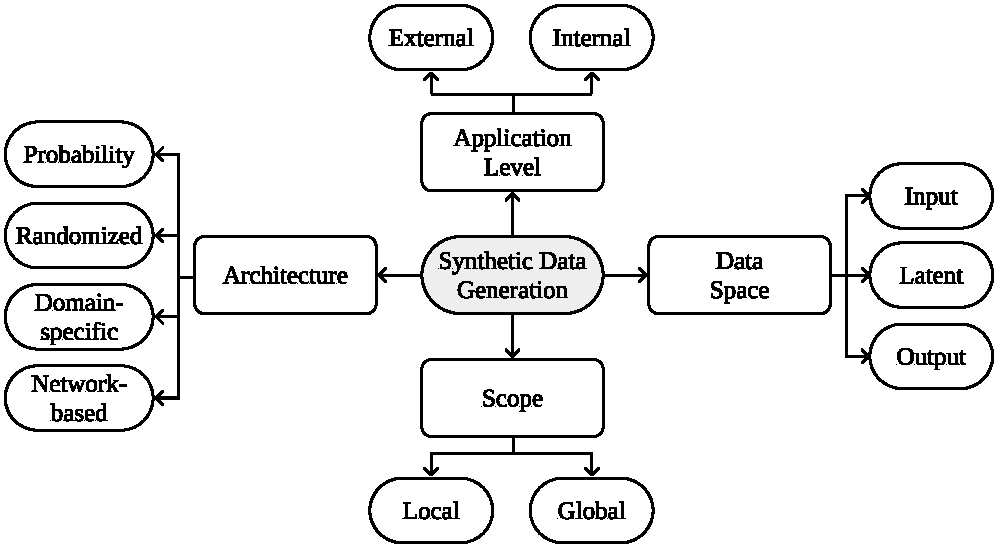
\includegraphics[width=.95\linewidth]{figures/synthetic-data-review/data-generation-taxonomy}
    \caption{General taxonomy of data generation mechanisms proposed in this
        paper.
    }~\label{fig:data-generation-taxonomy}
\end{figure}

Throughout the analysis of the different types of generation mechanisms, all
relevant methods were characterized using this taxonomy and listed in
Table~\ref{tbl:generators}.

\begingroup\small
\begin{longtable}{rcccccccc}
    \caption[Summary of the synthetic data generation methods discussed in
    this work.]{Summary of the synthetic data generation methods discussed in
    this work. A field containing ``---'' indicates that the it is either
    not applicable to the corresponding method, and/or applies its own unique
    approach.}
    \label{tbl:generators}\\
    \toprule
               Algorithm & ML Problem & Type &  Architecture & Level &  Data
               Space & Scope \\
    \midrule
    \endfirsthead
    \caption[]{Summary of the synthetic data generation methods discussed in
    this work. A field containing ``---'' indicates that the it is either
    not applicable to the corresponding method, and/or applies its own unique
    approach.} \\
    \toprule
               Algorithm & ML Problem & Type &  Architecture & Level &  Data
               Space & Scope \\
    \midrule
    \endhead
    \midrule
    \multicolumn{9}{r}{{Continued on next page}} \\
    \midrule
    \endfoot
    
    \bottomrule
    \endlastfoot
    SDV~\cite{patki2016synthetic} & Anon. & PDF & Probabilistic & External & Input & Global \\
    MST~\cite{mckenna2021winning} & DP & PGM & Probabilistic & External & Input & Global \\
    MWEM~\cite{hardt2012simple} & DP & Other & Probabilistic & External & Input & Global \\
    MWEM-PGM~\cite{mckenna2019graphical} & DP & PGM & Probabilistic & External & Input & Global \\
    PrivBayes~\cite{zhang2017privbayes} & DP & PGM & Probabilistic & External & Input & Global \\
    DPGAN~\cite{xie2018differentially} & DP & GAN & Network & External & Latent & Global \\
    DPCTGAN~\cite{rosenblatt2020differentially} & DP & GAN &  Network & External & Latent & Global \\
    PATE-GAN~\cite{jordon2018pate} & DP & GAN & Network & External & Lat. + Out. & Global \\
    PATECTGAN~\cite{rosenblatt2020differentially} & DP & GAN & Network & External & Lat. + Out. & Global \\
    FEM~\cite{vietri2020new} & DP & Perturb. & Probabilistic & External & Input & Global \\
    RAP~\cite{aydore2021differentially} & DP & Perturb. & Probabilistic & External & Input & Global \\
    PDF~\cite{de2019formal, suciu2011probabilistic} & --- & PDF & Probabilistic & External & Input & Global \\
    Kamino~\cite{ge2021kamino} & DP & PDF & Probabilistic & External & Input & Global \\
    RON-GAUSS~\cite{chanyaswad2019ron} & DP & PDF & Probabilistic & Internal & Latent & Global \\
    HDMM~\cite{mckenna2018optimizing} & DP & Perturb. & Probabilistic & External & Input & Global \\
    DualQuery~\cite{gaboardi2014dual} & DP & Other & Probabilistic & External & Input & Global \\
    ROS(E)~\cite{menardi2014training} & Ovs & Perturb. & Randomized & External & Input & Local \\ 
    SMOTE~\cite{Chawla2002} & Ovs & Linear & Randomized & External & Input & Local \\
    SMOTENC~\cite{Chawla2002} & Ovs & Linear & Randomized & External & Input & Local \\
    SMOTEN~\cite{Chawla2002} & Ovs & --- & --- & External & Input & Local \\
    Borderline-SMOTE~\cite{Han2005} & Ovs & Linear & Randomized & External & Input & Local \\
    G-SMOTE~\cite{Douzas2019} & Ovs & Geometric & Randomized & External & Input & Local \\
    ADASYN~\cite{HaiboHe2008} & Ovs & Linear & Randomized & External & Input & Local \\
    KernelADASYN~\cite{tang2015kerneladasyn} & Ovs & PDF & Probabilistic & External & Input & Local \\
    MOKAS~\cite{lin2017minority} & Ovs & Other & Network & External & Latent & Global \\
    SOMO~\cite{Douzas2017} & Ovs & Linear & Net.+Rand. & External & Input & Global \\
    G-SOMO~\cite{douzas2021g} & Ovs & Geometric & Net.+Rand. & External & Input & Global \\
    GMM-SENN~\cite{xing2022predict} & Ovs & PDF & Probabilistic & External & Input & Global \\
    GMF-SMOTE~\cite{xu2022synthetic} & Ovs & Linear & Randomized & External & Input & Global \\
    C-VAE~\cite{dai2019generative} & Ovs & AE & Network & External & Latent & Global \\
    Safe-level SMOTE~\cite{bunkhumpornpat2009safe} & Ovs & Linear & Randomized & External & Input & Local \\
    LR-SMOTE~\cite{liang2020lr} & Ovs & Linear & Randomized & External & Input & Global \\
    K-means SMOTE~\cite{Douzas2018} & Ovs & Linear & Randomized & External & Input & Global\\
    DBSMOTE~\cite{bunkhumpornpat2012dbsmote} & Ovs & Linear & Randomized & External & Input & Local\\
    CGAN~\cite{douzas2018effective} & Ovs & GAN & Network & External & Latent & Global \\
    K-means CTGAN~\cite{an2021k} & Ovs & GAN & Network & External & Latent & Global \\
    SMOTER~\cite{torgo2013smote} & Ovs + Reg & Linear & Randomized & External & Input & Local \\
    G-SMOTER~\cite{camacho2022geometric} & Ovs + Reg & Linear & Randomized & External & Input & Local \\
    RACOG~\cite{das2014racog} & Ovs & PGM & Probabilistic & External & Input & Global \\
    wRACOG~\cite{das2014racog} & Ovs & PGM & Probabilistic & External & Input & Global \\
    RWO~\cite{zhang2014rwo} & Ovs & PGM & Probabilistic & External & Input & Global \\
    PDFOS~\cite{gao2014pdfos} & Ovs & PDF & Probabilistic & External & Input & Global \\
    Mixup~\cite{zhang2018mixup} & DA & Linear & Randomized & External & In.+Out. & Local \\
    M-Mixup~\cite{verma2019manifold} & DA & Linear & Network & Internal & Lat.+Out. & Global \\
    NL-Mixup~\cite{guo2020nonlinear} & DA & Geometric & Randomized & External & In.+Out. & Local \\
    AE-DA~\cite{feng2020autuencoder} & DA & AE & Network & External & In./Lat.+Out. & Local \\
    MODALS~\cite{cheung2020modals} & DA & --- & Network & Internal & Latent & Global \\
    LSI~\cite{liu2018data} & DA & AE & Network & External & Lat.+Out. & Global \\
    Gibbs~\cite{fakoor2020fast} & DA & PGM & Probabilistic & External & Input & Global \\
    MedGAN~\cite{armanious2020medgan} & DA & GAN & Network & External & Latent & Global \\
    GANBLR~\cite{zhang2021ganblr} & DA & PGM & Probabilistic & External & Input & Global \\
    Table-GAN~\cite{park2018data} & DA & GAN & Network & External & Latent & Global \\
    CTGAN~\cite{xu2019modeling} & DA & GAN & Network & External & Latent & Global \\
    TVAE~\cite{xu2019modeling} & DA & AE & Network & External & Latent & Global \\
    AE~\cite{delgado2021deep} & DA & AE & Network & External & Latent & Global \\
    InfoMixup~\cite{Kim2021} & AL & Linear & Network & Internal & Lat.+Out. & Global \\
    VAEACGAN~\cite{tran2019bayesian} & AL & AE & Network & Internal & Latent & Global\\
    AL-G-SMOTE~\cite{Fonseca2021al} & AL & Geometric & Randomized & Internal & Input & Local\\
    DAE~\cite{rasmus2015semi} & Semi-SL & AE & Network & Internal & Input & Global \\ 
    $\Pi$-model~\cite{samuli2017temporal} & Semi-SL & Perturb. & Randomized & Internal & In.+Lat. & Local \\
    Mean Teacher~\cite{tarvainen2017mean} & Semi-SL & Perturb. & Randomized & Internal & In.+Lat. & Local \\
    ICT~\cite{verma2022interpolation} & Semi-SL & Linear & Randomized & Internal & Input & Local \\
    Mixmatch~\cite{berthelot2019mixmatch} & Semi-SL & Linear & Randomized & Internal & Input & Local \\
    SDAT~\cite{fang2022semi} & Semi-SL & AE+PDF & Net.+Prob. & Internal & Latent & Global \\
    MCoM~\cite{li2022mcom} & Semi-SL & Linear & Randomized & Int.+Ext. & Inp.+Lat. & Global \\
    C-Mixup~\cite{darabi2021contrastive} & Semi/Self-SL & AE+Lin. & Net+Rand.  & Internal & Latent & Global \\
    VIME~\cite{yoon2020vime} & Semi/Self-SL & Perturb. & Randomized & Internal & Input & Local \\
    SubTab~\cite{ucar2021subtab} & Self-SL & Perturb. & Rand.+Prob. & Internal & Input & Local \\
    Scarf~\cite{bahri2022scarf} & Self-SL & Perturb. & Randomized & Internal & Input & Local \\
    A-SFS~\cite{qiu2022sfs} & Self-SL & Perturb. & Randomized & Internal & Input & Local \\
\end{longtable}
\endgroup


\section{Algorithmic applications}\label{sec:algorithmic-applications}

In this section, we discuss the data generation mechanisms for the different
contexts where they are applied. We emphasize the constraints in each problem
that condition the way generation mechanisms are used. The literature search
was conducted with the Google Scholar database, using multiple keywords
related to each learning problem. Additional studies were collected by
checking the citing and cited articles of each study found initially. The
related work discussed in these studies was used to check for additional missing
methods. Although a larger preference was given to studies published in or
after 2019, our analysis includes relevant papers from previous years,
including seminal/classical publications in the field. All the steps involved
in the literature collection were conducted manually and individually for each
learning problem.

\subsection{Privacy}\label{sec:data-privacy}

Synthetic data generation is a technique used to produce synthetic, anonymized
versions of datasets~\cite{dankar2021fake}. It is considered a good approach
to share sensitive data without compromising significantly a given data mining
task~\cite{taub2018differential, park2018data}. Dataset anonymization via synthetic
data generation attempts to balance disclosure risk and data utility in the
final synthetic dataset. The goal is to ensure observations are not
identifiable and the relevant data mining tasks are not
compromised~\cite{singh2017aggregating, li2018privacy}.

The generation of synthetic datasets allows a more flexible approach to
implement ML tasks. To do this, it is important to guarantee that sensitive
information in $\mathcal{D}$ is not leaked into $\mathcal{D}^s$. Differential
privacy (DP), a formalization of privacy, offers strict theoretical privacy
guarantees~\cite{rosenblatt2020differentially}. A differentially private
generation mechanism produces a synthetic dataset, regulated by the privacy
parameter $\epsilon$, with statistically indistinguishable results when using
either $\mathcal{D}$ or neighboring datasets $\mathcal{D}' = \mathcal{D}
\backslash \{x\}$, for any $x \in \mathcal{D}$. A synthetic data generation
model ($f_{gen}$) guarantees $(\epsilon, \delta)$-differential privacy if
$\forall S \subseteq Range(f_{gen})$ all $\mathcal{D}, \mathcal{D}'$ differing
on a single entry~\cite{hardt2012simple}:

\begin{equation}
    Pr[f_{gen}(\mathcal{D}) \in S] \le e^{\epsilon} \cdot
    Pr[f_{gen}(\mathcal{D}') \in S] + \delta
\end{equation}
 
In this case, $\epsilon$ is a non-negative number defined as the privacy
budget. A lower $\epsilon$ guarantees a higher level of privacy but reduces
the utility of the produced synthetic data. DP synthetic data is especially
appealing since it is not affected by post-processing; any ML pipeline may be
applied on $\mathcal{D}^s$ while maintaining $(\epsilon, \delta)$-differential
privacy~\cite{dwork2014algorithmic}.

Choosing an appropriate DP synthetic data generation technique
is generally challenging and depends on the task to be developed (if known) and the domain. However,
marginal-based algorithms appear to perform well across various
tests~\cite{tao2021benchmarking}. A well-known method for the generation of DP
synthetic datasets is the combination of the Multiplicative Weights update
rule with the Exponential Mechanism (MWEM)~\cite{hardt2012simple}. MWEM is an
active learning-style algorithm that maintains an approximation of
$\mathcal{D}^s$. At each time step, MWEM selects the worst approximated query
(determined by a scoring function) using the Exponential Mechanism and
improves the accuracy of the approximating distribution using the
Multiplicative Weights update rule. A known limitation of this method is its
lack of scalability. Since this method represents the approximate data
distribution in datacubes, this method becomes infeasible for high-dimensional
problems~\cite{mckenna2019graphical}. This limitation was addressed with the
integration of a Probabilistic Graphical Model-based (PGM) estimation into
MWEM (MWEM-PGM) and a subroutine to compute and optimize the clique marginals
of the PGM, along with other existing privacy
mechanisms~\cite{mckenna2019graphical}. Besides MWEM, this method was used to
modify and improve the quality of other DP algorithms:
PrivBayes~\cite{zhang2017privbayes}, HDMM~\cite{mckenna2018optimizing} and
DualQuery~\cite{gaboardi2014dual}.

PrivBayes~\cite{zhang2017privbayes} addresses the curse of dimensionality by
computing a differentially private Bayesian Network (\textit{i.e.}, a type of
PGM). Instead of injecting noise into the dataset, they inject noise into the
lower-dimensional marginals. The high-dimensional matrix mechanism
(HDMM)~\cite{mckenna2018optimizing} mechanism is designed to efficiently
answer a set of linear queries on high-dimensional data, which are answered
using the Laplace mechanism. The DualQuery algorithm~\cite{gaboardi2014dual}
is based on the two-player interactions in MWEM and follows a similar
synthetic data generation mechanism as the one found in MWEM\@.

FEM~\cite{vietri2020new} follows a similar data generation approach as MWEM\@.
It also uses the exponential mechanism and replaces the multiplicative weights
update rule with the follow-the-perturbed-leader (FTPL)
algorithm~\cite{kalai2005efficient}. The Relaxed Adaptive Projection (RAP)
algorithm~\cite{aydore2021differentially} uses the projection
mechanism~\cite{nikolov2013geometry} to answer queries on the private dataset
using a perturbation mechanism and attempts to find the synthetic dataset that
matches the noisy answers as accurately as it can.

Kamino~\cite{ge2021kamino} introduces denial constraints in the data synthesis
process. It builds on top of the probabilistic database
framework~\cite{de2019formal, suciu2011probabilistic}, which models a
probability distribution function (PDF) and integrates denial constraints as
parametric factors, out of which the synthetic observations are sampled.
RON-GAUSS~\cite{chanyaswad2019ron} combines the random orthonormal (RON)
dimensionality reduction technique and synthetic data sampling using either a
Gaussian generative model or a Gaussian mixture model. The motivation for this
model stems from the \textit{Diaconis-Freedman-Meckes}
effect~\cite{meckes2012projections}, which states that most high-dimensional
data projections follow a nearly Gaussian distribution. Since RON-GAUSS
includes a feature extraction step (using RON) and the synthetic data
generated is not projected back into the input space, we consider RON-GAUSS an
internal approach to the ML pipeline.

The Maximum Spanning Tree (MST) algorithm~\cite{mckenna2021winning} is a
marginal estimation-based approach that produces differentially private data.
It uses the Private-PGM mechanism~\cite{mckenna2019graphical} that relies on
the PGM approach to generate synthetic data. PGM models are most commonly used
when it is important to maintain the pre-existing statistical properties and
relationships between features~\cite{young2009using}.

Another family of DP synthetic data generation techniques relies on the usage
of Generative Adversarial Networks (GAN). DPGAN~\cite{xie2018differentially}
modifies the original GAN architecture to make it differentially private by
introducing noise to gradients during the learning procedure. This approach
was also applied on a conditional GAN architecture directed towards tabular
data (CTGAN)~\cite{xu2019modeling}, which resulted in the
DPCTGAN~\cite{rosenblatt2020differentially} algorithm. Another type of
GAN-based DP data synthesis method is based on the combination of a GAN
architecture and the Private Aggregation of Teacher Ensembles
(PATE)~\cite{papernot2017semi} approach. Although the PATE method generates a
DP classifier, it served as the basis for PATE-GAN~\cite{jordon2018pate}, a DP
synthetic data generation mechanism. PATE-GAN replaces the discriminator
component of a GAN with the PATE mechanism, which guarantees DP over the
generated data. The PATE mechanism is used in the learning phase to train an
ensemble of classifiers to distinguish real from synthetic data. As a second
step, the predicted labels are passed (with added noise) to another
discriminator, which is used to train the generator network.

Finally, there are also popular synthetic data-based anonymization approaches to
perform anonymization without DP guarantees. For example, the Synthetic Data
Vault (SDV)~\cite{patki2016synthetic} anonymizes databases using Gaussian
copula models to generate synthetic data. However, this method allows the
usage of other generation mechanisms. A posterior extension of SDV was
proposed to generate data using a CTGAN~\cite{xu2019modeling} and to handle
sequential tabular data using a conditional probabilistic auto-regressive
neural network~\cite{zhang2022sequential}. 


\subsection{Regularization}\label{sec:regularization}

When the training data is clean, labeled, balanced, and sampled from a fixed
data source, the resulting ML classifier is expected to achieve good
generalization performance~\cite{benning2018modern}. However, if one or more
of these assumptions do not hold, the ML model becomes prone to
overfitting~\cite{Bartlett2021}. Regularization techniques are used to
address problems like overfitting, small training dataset, high
dimensionality, outliers, label noise, and catastrophic
forgetting~\cite{Halevy2009, Domingos2012, Salman2019, Xie2021}. One of
these techniques is data augmentation.
It is used to increase the size and variability of a training dataset, by
producing synthetic observations~\cite{Van2001, Wong2016}. Since it is applied
at the data level, it can be used for various types of problems and
classifiers~\cite{Behpour2019}. Although data
augmentation is commonly used and extensively studied in computer
vision~\cite{Shorten2019} and natural language
processing~\cite{feng2021survey}, its research on tabular data is less common.

Mixup~\cite{zhang2018mixup} consists of a linear interpolation between two
randomly selected observations and their target feature values, $(x_i, y_i),
(x_j, y_j) \in \mathcal{D}_L$, such that given $\lambda \sim
\text{Beta}(\alpha,\alpha)$, $x^s = \lambda x_i + (1-\lambda) x_j$ and $y^s =
\lambda y_i + (1-\lambda) y_j$, where $\alpha$ is a predetermined
hyperparameter. This method was the source of Manifold Mixup
(M-Mixup)~\cite{verma2019manifold}. It generates synthetic data in the latent
space of a neural network classifier's hidden layers. Another Mixup-based
data augmentation approach, Nonlinear Mixup
(NL-Mixup)~\cite{guo2020nonlinear}, applies a nonlinear interpolation policy.
In this case, $\Lambda$ is a set of mixing policies sampled from a beta
distribution applied to each feature. This approach modifies the original
mixup approach to generate data within a hyperrectangle/orthotope: $x^s =
\Lambda \odot x_i + (1-\Lambda) \odot x_j$, where $\odot$ denotes the Hadamard
product.

\cite{feng2020autuencoder} proposed an autoencoder-based data augmentation
(AE-DA) approach where the training of the autoencoder is done for each target
class, non-iteratively, which reduces the amount of time required compared to
the batch processing approach. The decoding weights of an autoencoder are
scaled and linearly combined with an observation from another class using a
coefficient that follows a beta distribution. The latter step varies from
typical interpolation-based approaches since this coefficient is usually
drawn from a uniform distribution.

The Modality-Agnostic Automated Data Augmentation in the Latent Space model
(MODALS)~\cite{cheung2020modals} leverages on the concept discussed
by~\cite{DeVries2017}, as well as the Latent Space Interpolation
method (LSI)~\cite{liu2018data} and M-Mixup~\cite{verma2019manifold}.
However, MODALS introduces a framework for data augmentation internally. It
contains a feature extraction step, trained using a combination of adversarial
loss, classification loss, and triplet loss, where latent space generation
mechanisms are applied. The classifier is trained using the original and the
synthetic observations generated in the latent space. In this study, the
authors discuss the difference transform augmentation method (among others already
described in this study). It generates within-class synthetic data by
selecting a $x^c$ and two random observations within the same class, $x_i,
x_j$, to compute $x^s = x^c + \lambda (x_i-x_j)$. In addition, they also
experiment with Gaussian noise and Hard example extrapolation, determined by
$x^s = x^c + \lambda (x^c-\mu)$, where $\mu$ is the mean of the observations
within a given class.

In the model distillation approach proposed in~\cite{fakoor2020fast} the
student model is trained with synthetic data generated with Gibbs sampling.
Although Gibbs sampling is infrequently used in recent literature, two
oversampling methods using Gibbs sampling appear to achieve state-of-the-art
performance~\cite{das2014racog}. However, probabilistic-based approaches for
data augmentation are uncommon; there are some methods proposed for the more
specific case of oversampling, but no more related methods for data
augmentation were found.

A well-known approach to GAN-based data augmentation is
Table-GAN~\cite{park2018data}. It utilizes the vanilla GAN approach to the
generation of synthetic data. However, vanilla GAN does not allow the
controlled generation of synthetic data given conditional attributes such as
the target feature values in supervised learning tasks and may be the cause
for aggravated categorical feature imbalance. These limitations were addressed
with the CTGAN~\cite{xu2019modeling} algorithm, which implements the
conditional GAN approach to tabular data. Another GAN-based architecture,
MedGAN~\cite{armanious2020medgan}, can also be adapted for tabular data and is
used as a benchmark in related studies (\textit{e.g.},~\cite{xu2019modeling,
zhang2021ganblr}). When compared to the remaining GAN-based approaches,
MedGAN's architecture is more complex and generally underperforms in the
experiments found in the literature. The GANBLR~\cite{zhang2021ganblr}
modifies vanilla GAN architectures with a Bayesian network as both generator
and discriminator to create synthetic data. This approach benefits from its
interpretability and reduced complexity while maintaining state-of-the-art
performance across various evaluation criteria.

Another less popular approach for network-based synthetic data generation
is
autoencoder architectures. TVAE, proposed in~\cite{xu2019modeling} achieved
state-of-the art performance.  It consists of the VAE algorithm with an
architecture modified for tabular data (\textit{i.e.}, 1-dimensional).
However, as discussed by the authors, this method contains limitations since
it is difficult to achieve DP with AE-based models since they access the
original data during the training procedure, unlike GANs.
\cite{delgado2021deep} studies the impact of data augmentation on supervised
learning with small datasets. The authors compare four different AE
architectures: Undercomplete, Sparse, Deep, and Variational AE\@. Although all
of the tested AE architectures improved classification performance, the deep
and variational autoencoders were the best overall performing models.

\subsection{Oversampling}\label{sec:oversampling}

Since most supervised ML classifiers are designed to expect classes with
similar frequencies, training them over imbalanced datasets can result in
limited classification performance.  With highly skewed distributions in
$\mathcal{D}_L$, the classifier’s predictions tend to be biased towards
overrepresented classes~\cite{Fonseca2021}. For example, one can
predict correctly with over 99\% accuracy whether credit card accounts were
defrauded using a constant classifier. One way to address this issue is
via oversampling~\cite{Douzas2019rs}, which can
be considered a specific setting of data augmentation.
It is an appropriate technique when, given a set of $n$ target
classes, there is a collection $C_{maj}$ containing the majority class
observations and $C_{min}$ containing the minority class observations such
that $\mathcal{D}_L = \bigcup^n_{i=1} C_i$. The training dataset
$\mathcal{D}_L$ is considered imbalanced if $|C_{maj}| > |C_{min}|$.
An oversampler is expected to generate a $\mathcal{D}_L^s = \bigcup^n_{i=1} C_i^s$
that guarantees $|C_i \cup C_i^s| = |C_{maj}|, \forall i \in \{1, \ldots,
n\}$. The model $f_\theta$ will be trained using an artificially balanced
dataset $\mathcal{D}_L' = \mathcal{D}_L \cup \mathcal{D}_L^s$.

Random Oversampling (ROS) is considered a classical approach to oversampling.
It oversamples minority classes by randomly picking samples with replacement.
It is a bootstrapping approach that, if generated in a smoothed manner
(\textit{i.e.}, by adding perturbations to the synthetic data), is also
known as Random Oversampling Examples (ROSE)~\cite{menardi2014training}.
However, the random duplication of observations often leads to
overfitting~\cite{Krawczyk2016}.

The Synthetic Minority Oversampling Technique (SMOTE)~\cite{Chawla2002}
attempts to address the data duplication limitation in ROS with a two-stage 
data generation mechanism:

\begin{enumerate}

    \item Selection phase. A minority class observation, $x^c \in C_{min}$,
        and one of its $k$-nearest neighbors, $x^{nn} \in C_{min}$, are
        randomly selected.

    \item Generation phase. A synthetic observation, $x^s$, is generated along
        a line segment between $x^c$ and $x^{nn}$: $x^s = \alpha x^c +
        (1-\alpha)x^{nn}, \alpha \sim \mathcal{U}(0, 1)$.

\end{enumerate}

Although the SMOTE algorithm addresses the limitations in ROS, it brings other
problems, which motivated the development of several SMOTE-based
variants~\cite{Douzas2019}: (1) it introduces noise when a noisy
minority class observation is assigned to $x^c$ or $x^{nn}$, (2) it
introduces noise when $x^c$ and $x^{nn}$ belong to different minority-class
clusters, (3) it introduces near duplicate observations when $x^c$ and
$x^{nn}$ are too close and (4) it does not account for within-class
imbalance (\textit{i.e.}, different input space regions should assume
different importance according to the concentration of minority class
observations).

Borderline-SMOTE~\cite{Han2005} modifies SMOTE's selection
mechanism. It calculates the $k$-nearest neighbors for all minority class
observations and selects the ones that are going to be used as $x^c$ in the
generation phase. An observation is selected based on the number of neighbors
belonging to a different class, where the observations with no neighbors
belonging to $C_{min}$ and insufficient number of neighbors belonging to
$C_{maj}$ are not considered for the generation phase. This approximates the
synthetic observations to the border of the expected decision boundaries.
Various other methods were proposed since then to modify the selection mechanism,
such as K-means SMOTE~\cite{Douzas2018}. This approach addresses
within-class imbalance and the generation of noisy synthetic data by
generating data within clusters. The data generation is done according to each
cluster's imbalance ratio and dispersion of minority class observations.
DBSMOTE~\cite{bunkhumpornpat2012dbsmote} also modifies the selection strategy
by selecting as $x^c$ the set of core observations in a DBSCAN clustering
solution.

The Adaptive Synthetic Sampling approach (ADASYN)~\cite{HaiboHe2008} uses a
comparable approach to Borderline-SMOTE\@. It calculates the ratio of
non-minority class observations within the $k$-nearest neighbors of each $x
\in C_{min}$. The number of observations to be generated using each $x \in
C_{min}$ as $x^c$ is determined according to this ratio; the more non-minority
class neighbors an observation contains, the more synthetic observations are
generated using it as $x^c$. The generation phase is done using the linear
mechanism in SMOTE\@. However, this approach tends to aggravate the limitation
(1) discussed previously. A second version of this method,
KernelADASYN~\cite{tang2015kerneladasyn}, replaces the generation mechanism
with a weighted kernel density estimation. The weighing is done according to
ADASYN's ratio and the synthetic data is sampled using the calculated Gaussian
Kernel function whose bandwidth is passed as an additional hyperparameter.

Modifications to SMOTE's generation mechanism are less common and generally
attempt to address the problem of noisy synthetic data generation. Safe-level
SMOTE~\cite{bunkhumpornpat2009safe} truncates the line segment between $x^c$
and $x^{nn}$ according to a safe level ratio. Geometric-SMOTE
(G-SMOTE)~\cite{Douzas2019} generates synthetic data within a
deformed and truncated hypersphere to also avoid the generation of
near-duplicate synthetic data. It also modifies the selection strategy to
combine the selection of majority class observations as $x^{nn}$ to avoid the
introduction of noisy synthetic data. 

LR-SMOTE~\cite{liang2020lr} modifies both the selection and generation
mechanisms. The set of observations to use as $x^c$ contains the misclassified
minority class observations using an SVM classifier, out of which the
potentially noisy observations are removed. The k-means clustering method is
used to find the closest observations to the cluster centroids, which are used
as $x^c$. The observations with a higher number of majority class neighbors
are more likely to be selected as $x^{nn}$. Although the generation mechanism
synthesizes observations as a linear combination between $x^c$ and $x^{nn}$,
it restricts or expands this range by setting $\alpha \sim \mathcal{U}(0, M)$,
where $M$ is a ratio between the average euclidean distance of each cluster's
minority class observations to $x^c$ and the euclidean distance between $x^c$
and $x^{nn}$.

The Minority Oversampling Kernel Adaptive Subspaces algorithm
(MOKAS)~\cite{lin2017minority} adopts a different approach when compared to
SMOTE-based mechanisms. It uses the adaptive subspace self-organizing map
(ASSOM)~\cite{kohonen1996emergence} algorithm to learn sub-spaces
(\textit{i.e.}, different latent spaces for each unit in the SOM), out of
which synthetic data is generated. The synthetic data is generated using a
lower dimensional representation of the input data to ensure the reconstructed
data is different from the original observations. Overall, the usage of SOMs
for oversampling is uncommon. Another two examples of this approach,
SOMO~\cite{Douzas2017} and G-SOMO~\cite{douzas2021g} use a similar
approach as K-means SMOTE\@. In the case of G-SOMO, the SMOTE
generation mechanism is replaced by G-SMOTE's instead.

Oversampling using GMM was found in a few recently proposed algorithms.
GMM-SENN~\cite{xing2022predict} fits a GMM and uses its inverse weights to
sample data, followed by the application of SMOTEENN to leverage the Edited
Nearest Neighbors (ENN) methods as a means to reduce the noise in the training
dataset. The GMM Filtering-SMOTE (GMF-SMOTE)~\cite{xu2022synthetic} algorithm
applies a somewhat inverse approach; a GMM is used to detect and delete
boundary samples the synthetic data is generated with SMOTE.

The contrastive learning-based VAE approach proposed
in~\cite{dai2019generative}, designed for oversampling, was adapted from
the architecture proposed in~\cite{abid2019contrastive}. They address a
limitation found in most oversampling methods, where these methods focus
almost exclusively on the distribution of the minority class, while largely
ignoring the majority class distribution. Their VAE architecture uses two
encoders trained jointly, using both a majority and a minority class
observation. The synthetic observation is generated by sampling from one of
the sets of latent variables (which follows a Gaussian distribution) and
projecting it into the decoder.

Another set of network-based methods that fully replace SMOTE-based mechanisms
is GAN-based architectures. One example of this approach is
CGAN~\cite{douzas2018effective}. It uses an adversarial training approach to
generate data that approximates the original data distribution and is
indistinguishable from the original dataset (according to the adversarial
classifier). A more recent GAN-based oversampler, K-means CTGAN~\cite{an2021k}
uses a K-means clustering method as an additional attribute to train the
CTGAN\@. In this case, cluster labels allow the reduction of within-class
imbalance. These types of approaches benefit from learning the overall
per-class distribution, instead of using local information only. However, GANs
require more computational power to train, their performance is sensitive to
the initialization, and are prone to the ``mode collapse'' problem.

Statistical-based oversampling approaches are less common. Some methods, such
as RACOG and wRACOG~\cite{das2014racog} are based on Gibbs sampling,
PDFOS~\cite{gao2014pdfos} is based on probability density function estimations
and RWO~\cite{zhang2014rwo} uses a random walk algorithm. Although
oversampling for classification problems using continuous features appears as
a relatively well-explored problem, there is a general lack of research on
oversampling using nominal features or mixed data types (\textit{i.e.}, using
both nominal and continuous features) and regression problems.
SMOTENC~\cite{Chawla2002} introduces a SMOTE adaptation for mixed data
types. It calculates the nearest neighbors of $x^c$ by including in the
Euclidean distance metric the median of the standard deviations of the
continuous features for every nominal feature value that is different
between $x^c$ and $x^{nn}$. The generation is done using the normal SMOTE
procedure for the continuous features and the nominal features are determined
with their modes within $x^c$'s nearest neighbors. The
SMOTEN~\cite{Chawla2002} is an oversampling algorithm for nominal
features only. It uses the nearest neighbor approach proposed in
\cite{cost1993weighted} and generates $x^s$ using the modes of the features
in $x^c$'s nearest neighbors. Solutions to oversampling in regression problems
are generally also based on SMOTE, such as SMOTER~\cite{torgo2013smote} and
G-SMOTER~\cite{camacho2022geometric}.

% \subsection{Time-Series}
% % TODO: 
% % - Table with literature review references 
% 
% % A general description of time series data
% 
% Synsys~\cite{dahmen2019synsys} approaches time-series using both Hidden Markov
% and regression models. They show the method's effectiveness in the Healthcare
% domain with limited ground truth data by comparing it to models trained using
% only real data. A related model, Sensegen~\cite{alzantot2017sensegen}, uses an
% adversarial training approach to train an LSTM that predicts the parameters
% of Gaussian Mixture Models (GMM) at each time stamp, using real data as
% an input. Finally, the GMM estimations are used to sample synthetic data. 
% 
% 
% Generative adversarial networks in time series 
% 
% 
% Some of the methods previously discussed can also be used for time-series. For
% example, \citet{cheung2020modals} show improved performance with time-series
% data using MixUp and MODALS


\subsection{Active Learning}\label{sec:active-learning}

AL is an informed approach to data collection and labeling. In classification
problems, when $|\mathcal{D}_U| \gg |\mathcal{D}_L|$ and it is possible to
label data according to a given budget, AL methods will search for the most
informative unlabeled observations. Once labeled and included in the
training set, these observations are expected to improve the performance of
the classifier to a greater extent when compared to randomly selected
observations. AL is an iterative process where an acquisition function
$f_{acq}(x, f_\theta): \mathcal{D}_U \to \mathbb{R}$ computes a classification
uncertainty score for each unlabeled observation, at each iteration.
$f_{acq}$ provides the selection criteria based on the uncertainty scores,
$f_\theta$ and the labeling budget~\cite{Kim2021}.

One way to improve an AL process is via the generation of synthetic data,
since the generation of informative, labeled, synthetic observations reduces the amount
of data labeling required to achieve a certain classification performance. In
this case, synthetic data is expected to improve classification with a better
definition of the classifier's decision boundaries. This allows the allocation
of the data collection budget over a larger area of the input space. These
methods can be divided into AL with pipelined data augmentation approaches and
AL with within-acquisition data augmentation~\cite{Kim2021}. Pipelined
data augmentation is the more intuitive approach, where at each training phase
the synthetic data is produced to improve the quality of the classifier and is
independent of $f_{acq}$. In \cite{Fonseca2021al}, the pipelined
approach in tabular data achieves superior performance compared to the
traditional AL framework using the G-SMOTE algorithm and the oversampling
generation policy. Other methods, although developed and tested on image data,
could also be adapted for tabular data: in the Bayesian Generative Active Deep
Learning framework~\cite{tran2019bayesian} the authors propose VAEACGAN, which
uses a VAE architecture along with an auxiliary-classifier generative
adversarial network (ACGAN)~\cite{odena2017conditional} to generate synthetic
data.

The Look-Ahead Data Acquisition via augmentation algorithm~\cite{Kim2021}
proposes an acquisition function that considers the classification uncertainty
of synthetic data generated using a given unlabeled observation, instead of
only estimating the classification uncertainty of the unlabeled observation
itself. This approach considers both the utility of the augmented data and the
utility of the unlabeled observation. This goal is achieved with the data
augmentation method InfoMixup, which uses M-Mixup~\cite{verma2019manifold}
along with the distillation of the generated synthetic data using $f_{acq}$.
The authors additionally propose InfoSTN, although the original Spatial
Transform Networks (STN)~\cite{jaderberg2015spatial} were originally designed
for image data augmentation.


% \subsection{Few-shot Learning}~\label{sec:few-shot-learning}
% 
% Few-shot learning (FSL) techniques attempt to address the limitation of small
% training datasets. The goal is to improve ML algorithms' capability for
% generalization in the same way a human is able to generalize knowledge from
% few examples. FSL is typically used when labeled data is impossible or
% difficult to acquire due to privacy, safety or ethic
% issues~\cite{wang2020generalizing}.
% 
% Analysis of six feature space data augmentation techniques for few-shot
% learning~\cite{kumar2019closer}
% 
% FlipDA~\cite{zhou2021flipda}
% 
% Data generation can be used to address Few-shot learning in three
% ways~\cite{wang2020generalizing}: (1) transforming samples from the dataset,
% (2) transforming samples from a weakly labeled or unlabeled dataset, or (3)
% transforming samples from similar datasets.

\subsection{Semi-supervised Learning}\label{sec:semi-supervised-learning}

Semi-supervised learning (Semi-SL) techniques modify the learning phase of ML
algorithms to leverage both labeled and unlabeled data. This approach is used
when $|\mathcal{D}_U| \gg |\mathcal{D}_L|$ (similarly to AL settings), but
additional labeled data is too difficult to acquire. In recent years,
the research developed in this area directed much of its focus to neural
network-based models and generative learning~\cite{Van2020}. Overall,
Semi-SL can be distinguished between transductive and inductive methods. In
this section, we will focus on synthetic data generation mechanisms in
inductive, perturbation-based Semi-SL algorithms, applicable to tabular or
latent space data.

The ladder network~\cite{rasmus2015semi} is a semi-supervised learning
architecture that learns a manifold latent space using a Denoising
Autoencoder (DAE). The synthetic data is generated during the learning phase;
random noise is introduced into the input data and the DAE learns to predict
the original observation. Although this method was tested with image data,
DAE networks can be adapted for tabular data~\cite{sattarov2022explaining}.

The $\Pi$-model simultaneously uses both labeled and unlabeled data in the
training phase~\cite{samuli2017temporal}. Besides minimizing cross-entropy,
they add to the loss function the squared difference between two input-level
transformations (Gaussian noise and other image-specific methods) in the
network's output layer. Mean Teacher algorithm~\cite{tarvainen2017mean} built
upon the $\Pi$-model, which used the same types of augmentation. The
Interpolation Consistency Training (ICT)~\cite{verma2022interpolation} method
combined the mean teacher and the Mixup approach, where synthetic observations
are generated using only the unlabeled observations and their predicted label
using the teacher model. In Mixmatch~\cite{berthelot2019mixmatch}, the Mixup
method is used by randomly selecting any pair of observations and their true
labels (if it's a labeled observation) or predicted label (if it's unlabeled).

The Semi-SL Data Augmentation for Tabular data (SDAT)
algorithm~\cite{fang2022semi} uses an autoencoder to generate synthetic data
in the latent space with Gaussian perturbations. The Contrastive Mixup
(C-Mixup)~\cite{darabi2021contrastive} algorithm generates synthetic data
using the Mixup mechanism with observation pairs within the same target label.
The Mixup Contrastive Mixup algorithm (MCoM)~\cite{li2022mcom} proposes the
triplet Mixup method using three observations where $x^s = \lambda_ix_i +
\lambda_jx_j + (1-\lambda_i-\lambda_j)x_k$, where $\lambda_i, \lambda_j \sim
\mathcal{U}(0, \alpha)$, $\alpha \in (0, 0.5]$ and $x_i$, $x_j$ and $x_k$
belong to the same target class. The same algorithm also uses the M-Mixup
method as part of the latent space learning phase.


\subsection{Self-supervised Learning}\label{sec:self-supervised-learning}

Self-supervised learning (Self-SL), although closely related to Semi-SL,
assumes $\mathcal{D}_L = \emptyset$. These models focus
on representation learning using $\mathcal{D}_U$ via secondary learning
tasks, which can be adapted to multiple downstream
tasks~\cite{liu2021self}. This family of techniques allows the usage of raw,
unlabeled data, which is generally cheaper to acquire when compared to
processed, curated, and labeled data. Although not all Self-SL methods rely on
data augmentation (\textit{e.g.}, STab~\cite{hajiramezanali2022stab}), the
majority of state-of-the-art tabular Self-SL methods use data augmentation as
a central concept for the training phase.

The value imputation and mask estimation method (VIME)~\cite{yoon2020vime} is
a Semi-SL and Self-SL approach that introduces Masking, a tabular data
augmentation method. It is motivated by the need to generate corrupted,
difficult-to-distinguish synthetic data in a computationally efficient way for
Self-SL training. They replace with probability $p_m$ the feature values in $x_i$
with another randomly selected value of each corresponding feature. To do
this, the authors use a binomial mask vector $m=[m_1, \ldots, m_d]^\bot \in
\{0,1\}^d$, $m_j \sim \text{Bern}(p_m)$, observation $x_i$ and the noise vector
$\epsilon$ (\textit{i.e.}, the vector of possible replacement values). A
synthetic observation is produced as $x^s=(1-m) \odot x_i + m \odot \epsilon$.
A subsequent study that proposed the SubTab~\cite{ucar2021subtab}
framework presents a multi-view approach; analogous to cropping in image data
or feature bagging in ensemble learning. In addition, the authors propose an
extension of the masking approach proposed in VIME by introducing noise using
different approaches: Gaussian noise, swap-noise (\textit{i.e.}, the approach
proposed in VIME) and zero-out noise (\textit{i.e.}, randomly replace a
feature value by zero).

The Self-supervised contrastive learning using random feature corruption
method (Scarf)~\cite{bahri2022scarf} uses a similar synthetic data generation
approach as VIME. Scarf differs from VIME by using contrastive loss instead of
the denoising auto-encoder loss used in VIME. A-SFS~\cite{qiu2022sfs} is a
Self-SL algorithm designed for feature extraction. It achieved higher
performance compared to equivalent state-of-the-art augmentation-free
approaches such as Tabnet~\cite{arik2021tabnet} and uses the masking
generation mechanism described in VIME.


% STab~\cite{hajiramezanali2022stab} --- Augmentation free
% RegCLR~\cite{wang2022regclr}
% Tabnet~\cite{arik2021tabnet}
% SELF-LLP~\cite{liu2022self} --- image data


\section{Generation mechanisms}\label{sec:generation-mechanisms}

In this section, we provide a general description of the synthetic data
generation mechanisms found in the learning problems in
Section~\ref{sec:algorithmic-applications}.
Table~\ref{tbl:generation-mechanisms} summarizes the assumptions and usage of
the generation mechanisms across the selected works and learning problems.

\begingroup\small
\begin{longtable}{clcccccccc}
    \caption{Analysis of synthetic data generation mechanisms.}
    \label{tbl:generation-mechanisms}\\
    \toprule
        Type & Mechanism & Smoothness & Manifold & Priv. & Reg. & Ovs. & AL & Semi-SL & Self-SL \\
    \midrule
    \endfirsthead
    \caption[]{Analysis of synthetic data generation mechanisms.} \\
    \toprule
        Type & Mechanism & Smoothness & Manifold & Priv. & Reg. & Ovs. & AL & Semi-SL & Self-SL \\
    \midrule
    \endhead
    \midrule
    \multicolumn{9}{r}{{Continued on next page}} \\
    \midrule
    \endfoot
    
    \bottomrule
    \endlastfoot
    \multirow{5}{*}{Perturbation} 
        & Random         & \checkmark & \checkmark 
                         & $\times$ & $\times$ & \checkmark & $\times$ & $\times$ & $\times$ \\

        & Laplace        & \checkmark & \checkmark 
                         & \checkmark & $\times$ & $\times$ & $\times$ & $\times$ & $\times$ \\

        & Gaussian       & \checkmark & \checkmark 
                         & \checkmark & \checkmark & $\times$ & $\times$ & \checkmark & \checkmark \\

        & Swap-noise     & $\times$ & $\times$ 
                         & $\times$ & $\times$ & $\times$ & $\times$ & \checkmark & \checkmark \\

        & Zero-out noise & $\times$ & $\times$ 
                         & $\times$ & $\times$ & $\times$ & $\times$ & $\times$ & \checkmark \\

    \midrule
    \multirow{3}{*}{PDF} 
        & Gaussian Gen. & $\times$ & \checkmark 
                        & \checkmark & $\times$ & \checkmark & $\times$ & $\times$ & $\times$ \\

        & Gaussian Mix. & $\times$ & \checkmark 
                        & \checkmark & $\times$ & \checkmark & $\times$ & $\times$ & $\times$ \\

        & KDE           & $\times$ & \checkmark 
                        & $\times$ & $\times$ & \checkmark & $\times$ & $\times$ & $\times$ \\

    \midrule
    \multirow{3}{*}{PGM} 
        & Bayesian Net. & $\times$ & $\times$ 
                        & \checkmark & \checkmark & $\times$ & $\times$ & $\times$ & $\times$ \\

        & Gibbs         & $\times$ & $\times$ 
                        & $\times$ & \checkmark & \checkmark & $\times$ & $\times$ & $\times$ \\

        & Random Walk & $\times$ & $\times$
                      & $\times$ & $\times$ & \checkmark & $\times$ & $\times$ & $\times$ \\


    \midrule
    \multirow{6}{*}{Linear} 
        & Between-class Int.  & $\times$ & \checkmark   
                              & $\times$ & \checkmark & $\times$ & \checkmark & \checkmark & $\times$ \\

        & Within-class Int.   & \checkmark & \checkmark 
                              & $\times$ & \checkmark & \checkmark & \checkmark & \checkmark & $\times$ \\
        
        & Extrapolation       & \checkmark & \checkmark 
                              & $\times$ & \checkmark & \checkmark & $\times$ & $\times$ & $\times$ \\

        & Hard Extra.         & \checkmark & \checkmark 
                              & $\times$ & \checkmark & \checkmark & $\times$ & $\times$ & $\times$ \\

        & Inter.+Extra.       & \checkmark & \checkmark 
                              & $\times$ & $\times$ & \checkmark & $\times$ & $\times$ & $\times$ \\

        & Difference Transf.  & \checkmark & \checkmark 
                              & $\times$ & \checkmark & $\times$ & $\times$ & $\times$ & $\times$ \\


    \midrule
    \multirow{3}{*}{Geometric} 
        & Hypersphere & \checkmark & \checkmark 
                      & $\times$ & $\times$ & \checkmark & \checkmark & $\times$ & $\times$ \\

        & Triangular  & \checkmark & \checkmark
                      & $\times$ & $\times$ & $\times$ & $\times$ & \checkmark & $\times$ \\

        & Hyperrectangle & $\times$ & \checkmark 
                         & $\times$ & \checkmark & $\times$ & $\times$ & $\times$ & $\times$ \\
    \midrule
    \multirow{2}{*}{Neural nets.} 
        & GAN & $\times$ & $\times$ 
              & \checkmark & \checkmark & \checkmark & \checkmark & $\times$ & $\times$ \\

        & AE & $\times$ & $\times$ 
             & $\times$ & \checkmark & \checkmark & \checkmark & \checkmark & $\times$ \\
    \midrule
    \multirow{2}{*}{Others}
        & Exponential M. & $\times$ & $\times$
                         & \checkmark & $\times$ & $\times$ & $\times$ & $\times$ & $\times$ \\

        & Reconstruction err. & $\times$ & $\times$ 
                               & $\times$ & $\times$ & \checkmark & $\times$ & $\times$ & $\times$ \\
\end{longtable}
\endgroup


We focus on 2 key conditions for the data generation process, smoothness, and
manifold space (adapted from the background in~\cite{Van2020}). The
smoothness condition requires that if two observations $x_i, x_j$ are close,
then it's expected that $y_i, y_j$ have the same value.  The manifold
condition requires synthetic data generation to occur within local Euclidean
topological spaces. Therefore, a generation mechanism with the smoothness
requirement also requires a manifold, while the opposite is not necessarily
true.

In the remaining subsections, we will describe the main synthetic data
generation mechanisms found in the literature, based on the studies discussed
in Section~\ref{sec:algorithmic-applications}.

\subsection{Perturbation Mechanisms}

The general perturbation-based synthetic data generation mechanism is defined
as $x^s = x_i + \epsilon$, where $\epsilon$ is the noise vector sampled from a
certain distribution. The random perturbation mechanism can be thought of as
the non-informed equivalent of PGMs and PDFs. It samples $|\epsilon|$ values
from a uniform distribution, \textit{i.e.}, $e_i \sim \mathcal{U}(\cdot,
\cdot), \forall e_i \in \epsilon$, while the minimum and maximum values depend
on the context and level of perturbation desired, typically centered around
zero.

Laplace (commonly used in DP algorithms) and Gaussian perturbations sample
$\epsilon$ with $e_i \sim \text{Lap}(\cdot, \cdot)$ and $e_i \sim
\mathcal{N}(\cdot, \cdot)$, respectively. Within the applications found, in
the presence of categorical features, these methods tend to use n-way
marginals (also known as conjunctions or contingency
tables~\cite{gaboardi2014dual}) to ensure the generated data contains
variability in the categorical features and the distribution of categorical
feature values follows some given constraint. Although various other
distributions could be used to apply perturbations, the literature found
primarily focuses on introducing noise via uniform, Laplace, and Gaussian
distributions.

\begin{figure}
	\centering
	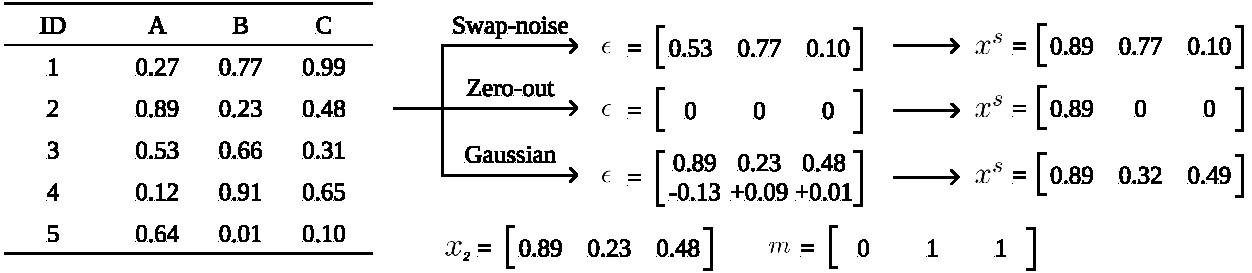
\includegraphics[width=.95\linewidth]{figures/synthetic-data-review/masking-example}
    \caption{Examples of synthetic observations generated with different
        masking approaches.
    }~\label{fig:masking-example}
\end{figure}

Masking modifies the original perturbation-based approach by introducing a
binomial mask vector, $m = [m_1, \ldots, m_d]^\bot \in \{0,1\}^d, m_i \sim
\text{Bern}(p_m)$ and the generation mechanism is defined as $x^s = (1 -
m)\odot x_i + m \odot \epsilon$~\cite{yoon2020vime}. The $\epsilon$ variable
is defined according to the perturbation used. The Gaussian approach generates
the noise vector as $\epsilon = x_i + \epsilon'$, where $e_i' \sim
\mathcal{N}(\cdot, \cdot), \forall e_i' \in \epsilon'$. The swap-noise
approach shuffles the feature values from all observations to form
$\epsilon$, while the zero-out noise approach sets all $\epsilon$ values to
zero. Intuitively, the masking technique modifies an observation's feature
values with probability $p_m$, instead of adding perturbations over the
entire observation. Figure~\ref{fig:masking-example} shows a visual depiction
of the masking technique.

\subsection{Probability Density Function Mechanisms}

The Gaussian generative model, despite being infrequently used when compared to the
remaining Probability Density Function mechanisms discussed in this subsection,
is an essential building block for these mechanisms. In particular, we focus
on the multivariate Gaussian approach, which follows near-Gaussian
distribution assumptions, which is rarely reasonable on the input space.
However, for high-dimensional data, it is possible to motivate this approach
via the \textit{Diaconis-Freedman-Meckes} effect~\cite{meckes2012projections},
which states that high-dimensional data projections generally follow a nearly
Gaussian distribution. The Gaussian generative model produces synthetic data
from a Gaussian distribution $x^s \sim \mathcal{N}(\mu, \Sigma)$, where $\mu
\in \mathbb{R}^d$ is a vector with the features' means and $\Sigma \in
\mathbb{R}^{d \times d}$ is the covariance matrix. It follows the following
density function~\cite{chanyaswad2019ron}:

\begin{equation}\label{eq:gaussian}
    f(x) =
    \frac{1}{\sqrt{(2\pi)^d\text{det}(\Sigma)}}\text{exp}\left(-\frac{1}{2}(x-\mu)^T\Sigma^{-1}(x-\mu)\right)
\end{equation}

Consequently, to define a Gaussian generative model it is only necessary to
estimate the dataset's mean and covariance matrix.

A Gaussian mixture model (GMM) comprises several Gaussian distributions that
aim to represent subpopulations within a dataset. Its training procedure
allows the model to iteratively learn the subpopulations using the Expectation
Maximization algorithm. A GMM becomes more appropriate than the Gaussian
generative model when the data is expected to have more than one
higher-density region, leading to a poor fit of unimodal Gaussian models.

Kernel Density Estimation (KDE) methods use a kernel function to estimate the
density of the dataset's distribution at each region of the input/latent
space. Despite the various kernel options, the Gaussian kernel is commonly
used for synthetic data generation~\cite{tang2015kerneladasyn}. The general
kernel estimator is defined as follows: 

\begin{equation}
    \hat{p}(x) = \frac{1}{N+h}
    \sum_{i=1}^{N}K\left(\frac{x-x_i}{h}\right)
\end{equation}

Where $N = |\mathcal{D}|$, $h$ is a smoothing parameter known as bandwidth and
$K$ is the kernel function. The Gaussian kernel is defined as follows:

\begin{equation}
    G_i(x) = K\left(\frac{x-x_i}{h} \right) = \frac{1}{(\sqrt{2\pi} h)^d} 
    \text{exp}\left(-\frac{1}{2}\frac{(x-x_i)^T(x-x_i)}{h}\right) 
\end{equation}

Therefore, the Gaussian KDE approach can also be expressed as $\hat{p}(x) =
\frac{1}{N+h}\sum_{i=1}^{N}G_i(x)$, while the data is sampled from the
estimated probability distribution. Figure~\ref{fig:pdf-example} shows a
visualization of the PDF mechanisms discussed, applied to a mock dataset.

\begin{figure}
	\centering
	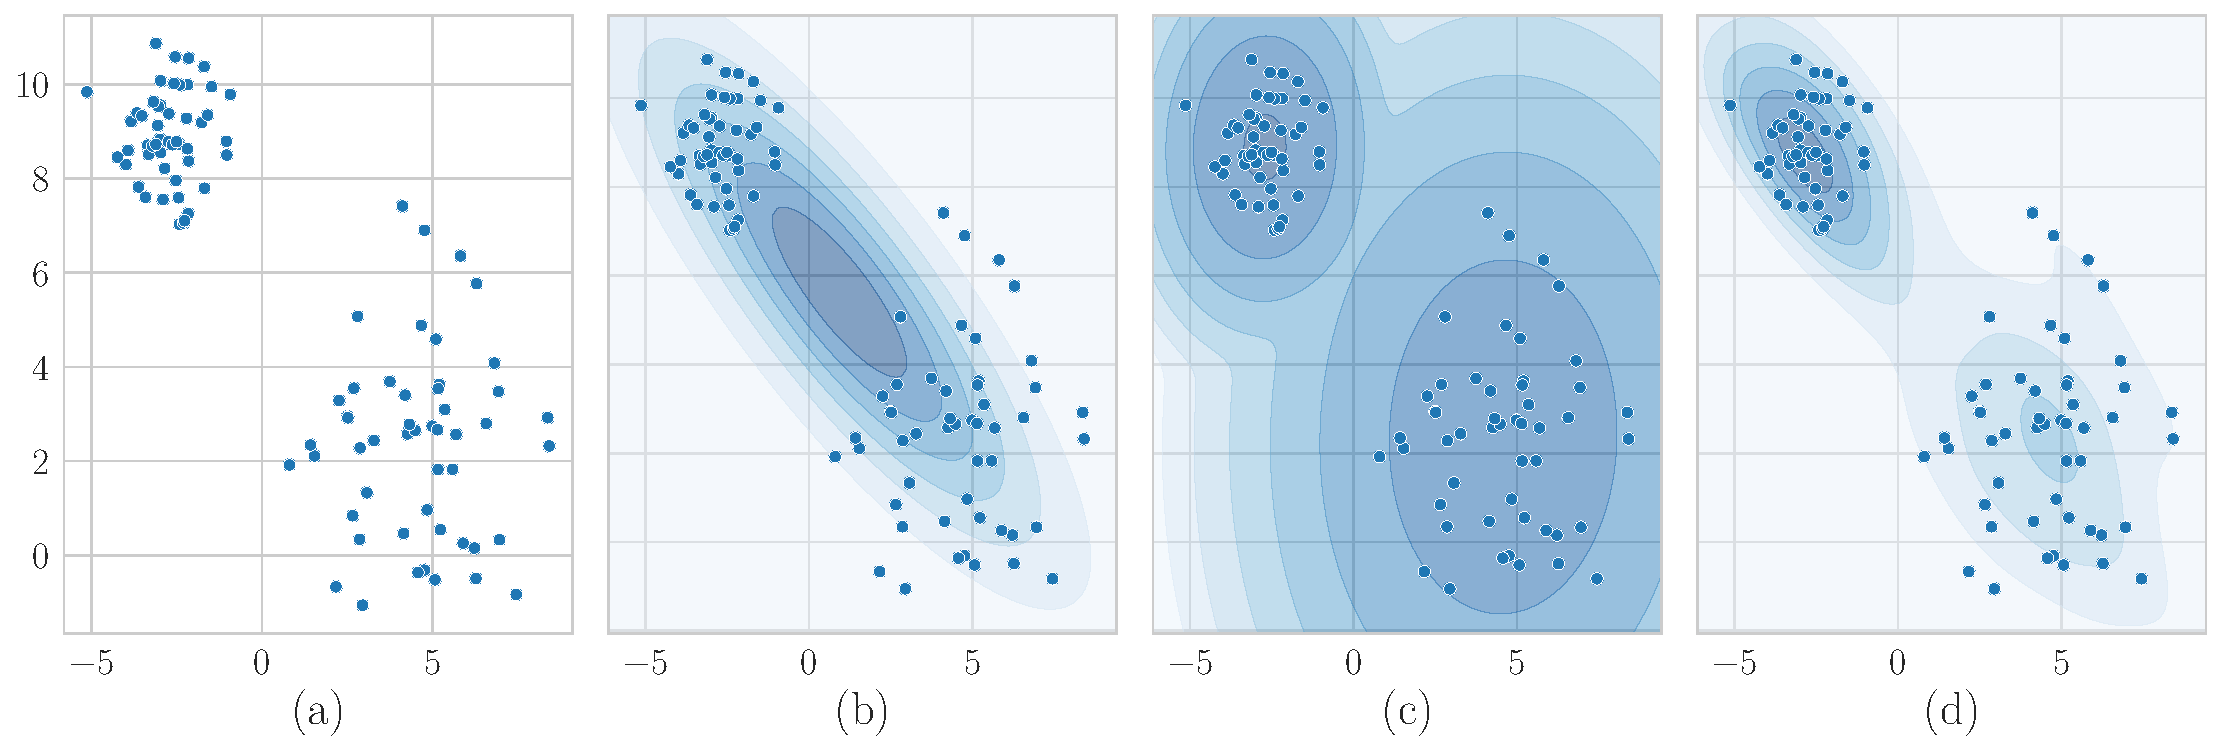
\includegraphics[width=.95\linewidth]{figures/synthetic-data-review/pdf-example}
    \caption[Examples of PDF mechanisms fitted to a mock dataset.]{%
        Examples of PDF mechanisms fitted to a mock dataset. Legend: (a)
        Original dataset, (b) Gaussian generative model, (c) Gaussian Mixture
        Model and (d) Gaussian Kernel Density Estimation.
    }~\label{fig:pdf-example}
\end{figure}

\subsection{Probabilistic Graphical Models}

A Bayesian network can be thought of as a collection of
conditional distributions. It represents the joint probability distribution
over the cross-product of the feature domains in $\mathcal{D}$. It is a
directed acyclic graph that represents $\mathcal{D}$'s features as nodes and
their conditional dependencies as directed edges. The set of features pointing
directly to feature $v \in V, d=|V|$ via a single edge are known as the parent
variables, $pa(v)$. A Bayesian network calculates $p(x)$ as the product of the
individual density functions, based on the conditional probabilities of the
parent variables:

\begin{equation}
    p(x) = \prod_{v \in V} p(x_v | x_{pa(v)})
\end{equation}

Since the construction of a directed acyclic graph can be labor intensive,
different ML approaches were developed for the learning of these
structures~\cite{yu2019dag}. Bayesian networks can be used for synthetic data
generation when the relationship between variables is known (or can be
learned) and when the data is high-dimensional, making the sampling process
non-trivial.

Random walk algorithms comprise the general process of iterating through a set
of random steps. Although uncommon, random walk approaches may be used to
sample data. The random walk approach described in \cite{zhang2014rwo} uses
the Gaussian noise mechanism over minority class observations to create
synthetic observations. The Gibbs sampling mechanism also performs a random
walk by iterating through sampled feature values.

Gibbs sampling is a Markov Chain Monte Carlo algorithm that iteratively
samples a synthetic observation's feature values. It is a suitable method to
sample synthetic data from a Bayesian network. The process starts with an
initial observation selected from $\mathcal{D}$, $x_0$, and is used to begin
the sampling process. In its original format, the sampling of each feature
value $v$ in $x^s_i$ is conditioned by $x^s_{i-1}$ and the feature values
already sampled from $x^s_i$, such that $x^s_{i, v} \sim p(x^s_{i, v} |
x^s_{i, 1}, \ldots, x^s_{i, v-1}, x^s_{i-1, v+1}, \dots, x^s_{i-1, d})$.
Therefore, Gibbs sampling is a special case of the Metropolis-Hastings
algorithm.

\subsection{Linear Transformations}

Linear interpolation mechanisms can be split into two subgroups: between and
within-class interpolation. Both mechanisms follow a similar approach; they
use a scaling factor $\lambda$, typically sampled from either
$\mathcal{U}(0,1)$ or $\text{Beta}(\alpha, \alpha)$: 

\begin{equation}~\label{eq:interpolation}
    x^s = \lambda x_i + (1-\lambda)x_j = x_j + \lambda(x_i - x_j)
\end{equation}

The within-class interpolation mechanism selects two observations from the
same class, while the between-class interpolation mechanism selects two
observations from different classes and also interpolates the one-hot encoded
target classes $y_i$ and $y_j$. However, the approach to select observations
might vary according to the ML task and data generation algorithm. For
example, most SMOTE-based methods select a center observation and a random
observation within its $k$-nearest neighbors belonging to the same class,
while the Mixup method selects two random observations, regardless of their
class membership.

\begin{figure}
	\centering
	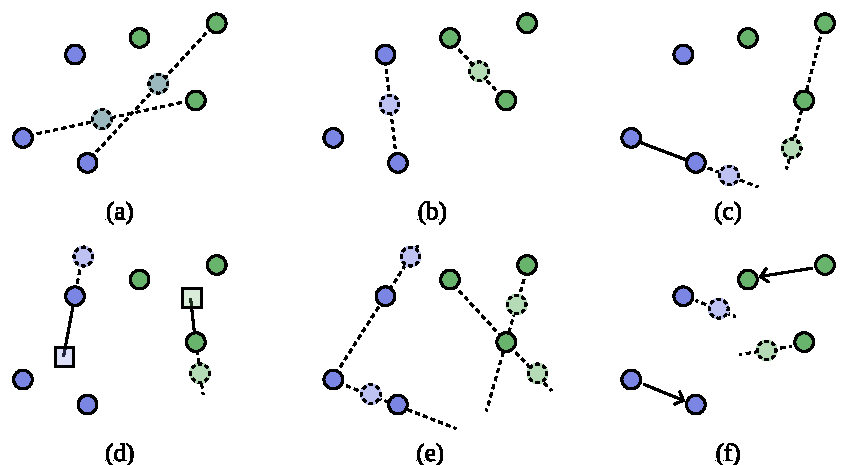
\includegraphics[width=.7\linewidth]{figures/synthetic-data-review/linear-transformations}
    \caption[Examples of linear transformation mechanisms.]{%
        Examples of linear transformation mechanisms. Legend: (a)
        Between-class interpolation, (b) Within-class interpolation, (c)
        Observation-based extrapolation, (d) Hard extrapolation, (e)
        Combination of interpolation and extrapolation and (f) Difference
        transform.
    }~\label{fig:linear-transformations}
\end{figure}

The observation-based linear extrapolation mechanism modifies
Equation~\ref{eq:interpolation} such that $x^s = x_i + \lambda(x_i - x_j)$,
while the hard extrapolation mechanism uses the mean of a class' observations,
$\mu^c$ and a randomly selected observation to generate $x^s = x_i^c +
\lambda(x_i^c - \mu^c)$. Some methods also combine both interpolation and
extrapolation. This can be achieved using Equation~\ref{eq:interpolation} and
modifying $\lambda$'s range to either decrease its minimum value below zero
or increase its maximum value above one.

The difference transform mechanism uses two observations to compute a
translation vector (multiplied by the scaling factor $\lambda$) and apply it
to a third observation:

\begin{equation}
    x^s = x_i + \lambda(x_j - x_k)
\end{equation}

Although there are various linear transformation mechanisms in the literature,
the majority of the studies applied linear interpolation mechanisms.
Within-class interpolation was frequently found in oversampling methods, while
between-class interpolation was found most often in regularization methods. A
depiction of the linear transformation mechanisms found in the literature
is presented in Figure~\ref{fig:linear-transformations}.

\subsection{Geometric Transformations}

Overall, geometric transformation mechanisms were not frequently found in the
literature. They are primarily used to develop Mixup or SMOTE-based variants.
Figure~\ref{fig:geometric-transformations} shows a visual example of the
related mechanisms.

The hypersphere mechanism generates data within a distorted, n-dimensional
hyper spheroid. It is formed using an observation to define the center of
the geometry and another to define its edge.
It is defined with two hyperparameters, the deformation
factor, $\alpha_{def} \in [0, 1]$, and the truncation factor, $\alpha_{trunc}
\in [-1, 1]$. The deformation factor deforms the hypersphere into an elliptic
shape, where $\alpha_{def}=1$ applies no deformation and $\alpha_{def}=0$
creates a line segment. The truncation factor limits the generation area of
the hyper spheroid within a subset of the hypersphere, where $\alpha_{trunc}=0$
applies no truncation, $\alpha_{trunc}=1$ uses the half of the area between
the two selected observations and $\alpha_{trunc}=-1$ uses the opposing area.
In Figure~\ref{fig:geometric-transformations}a, the two generation areas were
formed using approximately $\alpha_{trunc} = \alpha_{def} = 0.5$.

The triangular mechanism selects three observations to generate $x^s =
\lambda_ix_i + \lambda_jx_j + (1-\lambda_i-\lambda_j)x_k$, where $\lambda_i,
\lambda_j \sim \mathcal{U}(0, \alpha)$, $\alpha \in (0, 0.5]$. The
hyperrectangle mechanism uses an approach similar to
Equation~\ref{eq:interpolation}. However, the scaling factor is changed into a
scaling vector, $\Lambda = [\lambda_1,\dots,\lambda_d ] \in [0,1]^d, \lambda_i
\sim \text{Beta}(\alpha, \alpha)$, where $\alpha$ is a hyperparameter used to
define the Beta distribution. A synthetic observation is generated with $x^s =
\Lambda \odot x_i + (1-\Lambda) \odot x_j$, where $\odot$ denotes the Hadamard
product. This operation originates a generation area like the ones presented
in Figure~\ref{fig:geometric-transformations}c.

\begin{figure}
	\centering
	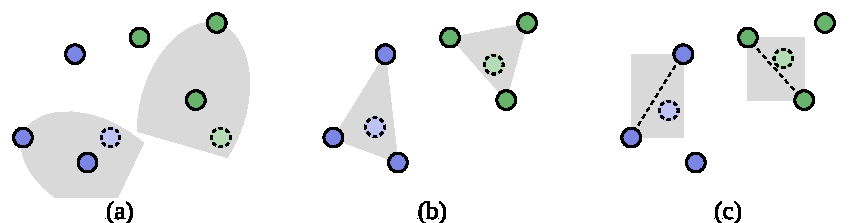
\includegraphics[width=.7\linewidth]{figures/synthetic-data-review/geometric-transformations}
    \caption[Examples of geometric transformation mechanisms.]{%
        Examples of geometric transformation mechanisms. Legend: (a)
        hypersphere mechanism, (b) triangular mechanism and (c)
        hyperrectangle mechanism.
    }~\label{fig:geometric-transformations}
\end{figure}

\subsection{Neural Networks}

Generative Adversarial Network (GAN) architectures are structured as a minimax
two-player game composed of two models, a generator, and a discriminator. Both
models are trained simultaneously throughout the learning phase, to learn to
generate data with similar statistical properties when compared to the
original data. The generative model captures the data distribution, while the
discriminator estimates the probability of an observation coming from the
training data. The goal of the generator model is to produce synthetic
observations that are capable of fooling the discriminator, making it
difficult for the discriminator to distinguish real from synthetic
observations. Although they were originally developed in an unsupervised
learning setting~\cite{goodfellow2020generative}, subsequent contributions
proposed GANs with several different architectures, for semi-SL, supervised
learning (for both regularization and oversampling), and reinforcement
learning.

An autoencoder (AE) is a type of neural network architecture that learns
manifold representations of an input space. These models are typically trained
by regenerating the input and are designed with a bottleneck in the hidden
layers that correspond to the learned latent space. It contains two parts,
an encoder, and a decoder. The encoder transforms the input data into
lower-dimensional representations (\textit{i.e.}, the latent space), while
the decoder projects these representations into the original input space.
Since it was first proposed~\cite{ackley1985learning}, many variants were
developed for multiple applications. However, based on the literature found,
the variational AE architecture appears to be the most popular approach.


\section{Evaluating the Quality of Synthetic Data
}\label{sec:evaluating-synthetic-data}

The vast majority of synthetic data generation models are evaluated on an ML
utility basis. Compared to research on the development of actual synthetic
data generation algorithms, there is a general lack of research on the
development of metrics to evaluate their quality beyond performance metrics
such as Overall Accuracy (OA) or F1-score.
% \footnote{\hl{For a more comprehensive
% analysis and definitions of frequently used supervised learning performance
% metrics, the reader is referred to}~\cite{seliya2009study}.} 
One motivation to
do this is the ability to anticipate the quality of the data for the target
task before training an ML classifier, which may be expensive and
time-consuming. This is a challenging problem since the usefulness of
synthetic data generators depends on the assumptions imposed according to
the dataset, domain, and ML problem~\cite{chundawat2022tabsyndex}. This
section focuses on the main evaluation approaches found in the literature
beyond classification performance, as well as recently proposed methods. For a
more comprehensive analysis of performance metrics for synthetic data
evaluation, the reader is referred to~\cite{dankar2022multi}
and~\cite{theis2016note}.

The GANBLR model~\cite{zhang2021ganblr} was evaluated on three aspects: (1) ML
utility, (2) Statistical similarity, and (3) Interpretability. In
\cite{xu2019modeling}, the authors evaluate the CTGAN and TVAE models using a
likelihood fitness metric (to measure statistical similarity) and ML efficacy
(\textit{i.e.}, utility). \cite{hittmeir2019utility} evaluate synthetic data
generators using a 2-step approach: Similarity comparison and data utility.
According to \cite{alaa2022faithful}, the evaluation of generative models
should quantify three key aspects of synthetic data:

\begin{enumerate}

    \item Fidelity. Synthetic observations must resemble real
        observations; 

    \item Diversity. Synthetic observations should cover $\mathcal{D}$'s
        variability;

    \item Generalization. Synthetic observations should not be copies of
        real observations;

\end{enumerate}

Ensuring these properties are met will secure the objectives defined in
Section~\ref{sec:problem-formulation}: $\mathbb{P}^s \approx
\mathbb{P}$ and $x_i \neq x_j \forall x_i \in \mathcal{D} \wedge x_j \in
\mathcal{D}^s$. However, this is a relatively recent consideration that was
not commonly found in the literature. The only study found to explicitly
address all three aspects was~\cite{alaa2022faithful}, although all other
studies and metrics discussed in Section~\ref{sec:quantitative-approaches}
address (implicitly or explicitly) at least one of these aspects.

The effective evaluation of synthetic data generation methods is a complex
task. Good performance on one evaluation method does not
necessarily imply a good performance on the primary ML task, results from
different evaluation methods seem to be independent, and evaluating the models
directly onto the target application is generally
recommended~\cite{theis2016note}. Therefore, each evaluation procedure must be
carefully implemented and adapted according to the use case.

\subsection{Quantitative approaches}~\label{sec:quantitative-approaches}

The Kullback-Leibler (KL) divergence (and equivalently the log-likelihood) is a
common approach to evaluate generative models~\cite{theis2016note}. Other
commonly used metrics, like Parzen window estimates, appear to be a generally
poor quality estimation method and are not recommended for most
applications~\cite{theis2016note}. KL divergence is defined as follows:

\begin{equation}
    D_{KL}(P||Q) = \sum_{x\in\mathcal{X}}P(x)\log{\frac{P(x)}{Q(x)}}
\end{equation}

Where $\mathcal{X}$ is a probability space, $P$ and $Q$ are estimated
probability distributions based on $\mathbb{P}$ and $\mathbb{P}^s$,
respectively. The KL divergence is a non-symmetric measurement that represents
how a reference probability distribution ($P$) differs from another
($Q$). A $D_{KL}$ close to zero means $Q$ is similar to $P$. However, metrics
like the KL divergence or the log-likelihood are generally difficult to
interpret, do not scale well for high dimensional data, and fail to
highlight model failures~\cite{alaa2022faithful}. Another related metric, used
in~\cite{zhao2021ctab}, is the Jensen-Shannon (JS) divergence. It consists of
a symmetrized and smoothed variation of the KL divergence. Having
$M=\frac{P+Q}{2}$, it is calculated as:

\begin{equation}
    D_{JS}(P||Q) = \frac{D_{KL}(P||M) + D_{KL}(Q||M)}{2}
\end{equation}

The Wasserstein Distance is another relevant metric to estimate the
distance between two distribution functions. It was also used to develop GAN
variants since it improves the stability in the training of
GANs~\cite{gulrajani2017improved, goncalves2020generation}.

In past literature, the propensity score was considered an appropriate
performance metric to measure the utility of masked data~\cite{woo2009global}.
This metric is estimated using a classifier (typically a logistic regression)
trained on a dataset with both the original and synthetic data, using as a
target the source of each observation (synthetic or original). The goal of
this classifier is to predict the likelihood of an observation being
synthetic. Therefore, this approach guarantees observation-level insights
regarding the faithfulness of each observation. \cite{woo2009global} suggest
a summarization of this metric, also defined as the propensity Mean Squared Error
(pMSE)~\cite{chundawat2022tabsyndex}:

\begin{equation}~\label{ep:propensity}
    U_p = pMSE = \frac{1}{N} \sum^N_{i=1}{(\hat{p}_i - c)}^2
\end{equation}

Where $N = |\mathcal{D} \cup \mathcal{D}^s|$, $c = \frac{|\mathcal{D}^s|}{N}$
and $\hat{p}_i$ is the estimated propensity score for observation $i$. When a
synthetic dataset is indistinguishable from real data, $pMSE$ will be close to
zero. Specifically, when the data source is indistinguishable, the expected
pMSE is given by~\cite{snoke2018general}:

\begin{equation}
    E(pMSE) = \frac{(k-1)(1-c)^2c}{N}
\end{equation}

Where $k$ is the number of parameters in the logistic regression model
(including bias). When the synthetic dataset is easily distinguishable from
the original dataset, $U_p$ will be close to ${(1-c)}^2$.
\cite{dankar2021fake}, established a generally consistent, weak negative
correlation between $U_p$ and OA\@.

\cite{chundawat2022tabsyndex} proposed TabSynDex to address the lack of
uniformity of synthetic data evaluation, which can also be used as a loss
function to train network-based models. It is a single metric evaluation
approach bounded within $[0,1]$ that consists of a combination of (1) the
relative errors of basic statistics (mean, median, and standard deviation), (2)
the relative errors of correlation matrices, (3) a pMSE-based index, (4) a
support coverage-based metric for histogram comparison and (5) the performance
difference in an ML efficacy-based metric between models trained on real and
synthetic data.

The three-dimensional metric proposed by~\cite{alaa2022faithful} presents an
alternative evaluation approach. It combines three metrics
($\alpha$-Precision, $\beta$-Recall, and Authenticity) for various application
domains. It extends the Precision and Recall metrics defined
in~\cite{sajjadi2018assessing} into $\alpha$-Precision and $\beta$-Recall,
which are used to quantify fidelity and diversity. Finally, the authenticity
metric is estimated using a classifier that is trained based on the distance
(denoted as $d$) between $x^s$ and its nearest neighbor in $\mathcal{D}$,
$x_{i^*}$; if $d(x^s, x_{i^*})$ is smaller than the distance between $x_{i^*}$
and its nearest neighbor in $\mathcal{D}\backslash \{x_{i^*}\}$, $x^s$ will
likely be considered unauthentic. This approach provides a threefold
perspective over the quality of $\mathcal{D}^s$ and allows a sample-level
analysis of the generator's performance. Furthermore, there is a relative
trade-off between the two metrics used to audit the generator and the
synthetic data; a higher $\alpha$-Precision score will generally correspond to
a lower Authenticity score and vice versa.

A less common evaluation approach is to attempt to replicate the results of
studies using synthetic data~\cite{el2020seven, benaim2020analyzing,
rosenblatt2022epistemic}. Another method is the computation of the
average distance among synthetic observations and their nearest neighbors
within the original dataset~\cite{hittmeir2019utility}. The Confidence
Interval Overlap and Average Percentage Overlap metrics may be used to
evaluate synthetic data specifically for regression
problems~\cite{khan2022utility, karr2006framework}.

\subsection{Visual and Qualitative approaches}

One of the qualitative approaches found in the literature is the comparison of
the features' distributions with synthetic data and the original data using
histogram plots~\cite{hittmeir2019utility}. This comparison can be
complemented with the quantification of these distribution
differences~\cite{el2020seven}. A complementary approach is the comparison of
correlation matrices via heat map plots~\cite{hittmeir2019utility}.

Another way to assess the quality of synthetic data is to evaluate
individual, synthetic data points and collect subjective
evaluations by domain experts~\cite{el2020seven}. The goal of such a test is to
understand whether domain experts are able to distinguish synthetic from real
data, which could be quantified with classification performance metrics. A low
classification performance implies synthetic data that is difficult to
distinguish from real data.

\section{Discussion}\label{sec:discussion}

The generation of tabular and latent space synthetic data has applications in
multiple ML tasks and domains. Specifically, we found six areas that were
shown to benefit from synthetic data: data privacy, regularization,
oversampling, active learning, semi-supervised learning, and self-supervised
learning. Synthetic data may be used either as an accessory task to improve
an ML model's performance over a primary task (\textit{e.g.},
regularization and oversampling), an intermediate task (\textit{e.g.}, feature
extraction), or as a final product itself (\textit{e.g.}, data anonymization).
The analysis of data generation algorithms for each relevant learning problem
led to the proposal of a general-purpose taxonomy primarily focused on the
underlying mechanisms used for data generation. We characterized every
algorithm discussed in this work into four categories: (1) architecture, (2)
application level, (3) data space, and (4) scope. The successful implementation
of synthetic data generation generally requires a few considerations:

\begin{enumerate}

    \item Ensuring the dataset's features are comprised within similar, fixed
        boundaries. For example, any method using a neighbors-based approach
        will rely on distance measurements (typically the Euclidean distance),
        which is sensitive to the scale of the data and a nearest-neighbors
        estimation may vary depending on whether the data was scaled \textit{a
        priori}. This can be achieved with data scaling. 

    \item Various generation mechanisms require a manifold. There are two
        approaches to address non-manifold input data: (1) Adopt methods
        sensitive to the presence of non-metric features, or (2) project the
        input data into a manifold (\textit{i.e.}, a latent space).

    \item The smoothness assumption is prevalent in linear and
        perturbation-based data generation mechanisms. If a classification
        problem has low class separation and it is difficult to solve, the choice in
        the design of the generator algorithm is also difficult. Generally,
        generation algorithms with a global scope might adapt better to
        classification problems with low separability. On the other hand,
        problems with higher separability might require a definition of more
        uniform decision boundaries to prevent overfitting, which can be
        achieved with generation algorithms with a local scope.

    \item Considering the trade-off between performance and computational
        power. It is generally understood that computationally-intensive
        approaches tend to produce synthetic data with higher quality. When
        trained properly, neural network mechanisms typically lead to
        synthetic data that is more difficult to distinguish compared to the
        remaining approaches. Geometric mechanisms have also achieved good
        results but often require careful tuning of their hyperparameters.
        Linear and perturbation mechanisms do not require much training and
        use fewer hyperparameters but have been known for often producing low
        diversity synthetic data (\textit{vis a vis} the original dataset).

\end{enumerate}

This work focused primarily on the mechanisms used to generate synthetic
observations; preprocessing, learning phase design, latent space learning, and
ML task-specific contributions were secondary objectives for analysis.
Consequently, understanding how the constraints within each task condition
the choice and design of the synthetic data generator is a subject of future
work.

Throughout the analysis of the literature, we identified six types of
generation mechanisms and discuss more specific methods used in classical and
state-of-the-art techniques. Techniques for data privacy via synthetic data
rely primarily on perturbation mechanisms, PDFs, PGMs, and Neural networks.
Regularization approaches frequently employ linear perturbation mechanisms.
Other less commonly used mechanisms are PGMs, Neural network approaches,
geometric, and perturbation mechanisms. Various Oversampling algorithms have
been proposed using each of the mechanisms found. However, the most prevalent
mechanisms used were linear-based. AL methods rarely employ synthetic data.
The few studies found employ primarily linear and geometric mechanisms, and a
minority used AE models for latent space augmentation. Most Semi-SL methods
used perturbation and linear mechanisms, while geometric mechanisms are rarely
used. All tabular Self-SL methods used perturbation mechanisms. 

% Recommendations for data evaluation
Designing an approach to measure the quality of synthetic data depends on the
target ML problem. A holistic evaluation approach for synthetic data should
consider the analysis of (1) ML utility, (2) Statistical similarity, and (3)
interpretability. The analysis of statistical similarity can be further
divided into (1) fidelity, (2) diversity, and (3) generalization.  However,
balancing the analysis between these three perspectives is not a
straightforward task. For example, duplicating a dataset to form a synthetic
dataset will result in the best possible fidelity and diversity, but bad
generalization. Overall, there is a paucity of research into the development
of comprehensive analyses of synthetic data, as well as understanding the
balance between the different types of analyses.


\section{Future Work}\label{sec:future-work}

As discussed throughout our analysis, it appears that synthetic data
generation research is generally isolated within ML problems and/or domains.
Given the breadth and complexity of input-level and latent-level data
generation mechanisms, it is increasingly important to find an \textit{a
priori} approach to efficiently determine appropriate data generation policies
and techniques. However, the complexity of this task is determined by various
factors: different data types, ML problems, model architectures, computational
resources, performance metrics, and contextual constraints.
Auto-augmentation and meta-learning aim to address this challenge and are
still subject to active research.

\textbf{Latent space learning.} It is understood that, if learned
properly, the latent space is expected to be convex and isotropic. In that
case, using linear generation techniques in the latent space would produce
synthetic data without introducing noise~\cite{cheung2020modals}. However, it
is unclear which types of model/architectures and training procedures
contribute to the learning of a good latent space according to the context.
Furthermore, we found a limited amount of research on tabular data
augmentation using auto-encoder architectures. Although there are studies
performing data augmentation on tabular data in various
domains~\cite{delgado2021deep}, defining the architecture and learning phase
of an AE is not an intuitive task. Generally, autoencoders are used to learn a
manifold for more complex data types. As long as the method used to generate
the latent space is appropriate, the methods discussed in this study could be
used in the latent space regardless of the type of data.

The quality of synthetic data generation in high-dimensional scenarios appears
as a prevailing limitation in various applications, especially within linear
and geometric mechanisms. This limitation can be addressed with dimensionality
reduction techniques~\cite{roccetti2021alternative}, as well as latent space
learning.  However, research on data generation in the latent space is mostly
focused on GAN architectures, which require significant computational power.
Other methods to learn manifold latent spaces could be explored to address
this limitation.

\textbf{Selection of generation mechanisms.} It remains an open question
which generation mechanisms, or types of
mechanisms, create better synthetic data~\cite{cheung2020modals}. Although
there is not necessarily a one-size-fits-all solution, a general set of rules
of thumb could be explored, such as understanding how certain characteristics
of a problem will affect the choice of the generation policy, which types of
mechanisms are more appropriate for different types of dataset, ML model
architecture, domains, and target ML problem, or the trade-offs between the
different types of generation mechanism. A better understanding of the
relationship between recently proposed methods for evaluating synthetic data
(as discussed in Section~\ref{sec:evaluating-synthetic-data}) and the
performance over the target ML problem might contribute to answering this question.
Furthermore, determining the use cases, quality, and general performance of
data generation on the input, latent, and output space should be further
developed. Finally, it is still unclear \textit{why} synthetic data generation
works for each of the ML tasks discussed. Research on this topic lacks depth
and fails to address the theoretical underpinnings~\cite{feng2021survey,
dao2019kernel}.

% data privacy
\textbf{Data privacy.} The evaluation of anonymization techniques lacks standardized,
objective, and
reliable performance metrics and benchmark datasets to allow an easier
comparison across classifiers to evaluate key aspects of data anonymization
(resemblance, utility, privacy, and performance). These datasets should contain
mixed data types (\textit{i.e.}, a combination of categorical, ordinal,
continuous, and discrete features) and the metrics should evaluate the
performance of different data mining tasks along with the anonymization
reliability. This problem appears to be universal across domains. For example,
\cite{hernandez2022synthetic} observed the lack of a universal method or
metric to report the performance of synthetic data generation algorithms for
tabular health records. Therefore, in order to facilitate the usage of these
techniques in industry domains, these benchmarks must also be
realistic. \cite{rosenblatt2020differentially} attempts to address this
problem by proposing a standardized evaluation methodology using standard
datasets and real-world industry applications.

% Regularization in supervised learning
\textbf{Regularization in supervised learning. }Unlike data privacy
solutions, studies on data augmentation techniques generally do not consider
the similarity/dissimilarity of synthetic data. The study of quality metrics
for supervised learning may reduce computational overhead and experimentation
time. Only one study related to the relationship between quality metrics
and performance in the primary ML task was found in~\cite{dankar2021fake},
which was done only for the pMSE metric.

\textbf{Consistency and interpretability.} Neural network mechanisms typically
involve a higher computational cost compared to the remaining types of
mechanisms. This problem is further aggravated by their inconsistent
performance, since different initializations may result in very different
performances. This problem may be observed in~\cite{douzas2018effective}. More
generally, representing training data in the latent space raises the
challenge of interpretability; the ability to interpret latent space
representations could guide the design of data generation techniques. 

\textbf{Ensembles of generation mechanisms.} In non-tabular data domains,
a common approach for data augmentation is the combination of several data
augmentation methods to increase the diversification of synthetic data. This
is true for both text classification~\cite{bayer2021survey} and image
classification~\cite{grill2020bootstrap}. However, for tabular data, no
studies were found that discuss the potential of ensembles of generation
mechanisms on tabular data, \textit{i.e.}, understanding how selecting with
different probabilities different generation mechanisms to generate synthetic
data would affect the performance of the primary ML task. The formalization
and analysis carried out in this work, regarding the different types of
synthetic data generation mechanisms and quality metrics for latent and
tabular synthetic data at an observation level, may facilitate this work.


% oversampling
\textbf{Oversampling.} Various oversampling methods have been proposed to
address imbalanced learning limitations. However, there is still a major
limitation in the literature regarding the oversampling of datasets with mixed
data types or with exclusively non-metric features at the input space. In
addition, research on oversampling using PDFs or PGMs is scarce.

\textbf{Tabular few-shot learning.} To the best of our knowledge,
research on few-shot learning for tabular data is infrequent. Few-shot
learning research using synthetic data generation techniques has been
extensively developed using image~\cite{cubuk2019autoaugment, zhao2019data}
and text data~\cite{zhou2021flipda}, but they are rarely adapted or tested for
tabular data. One of the few studies found achieved a good performance in both
few-shot and zero-shot learning through the adaptation of a Large Language
model for tabular data~\cite{hegselmann2022tabllm}. 

\textbf{Fairness and bias.} Oversampling does not seem to be a relevant
source of bias in behavioral research and does not appear to have an
appreciably different effect on results for directly versus indirectly
oversampled variables~\cite{hauner2014latent}. However, most oversampling
methods do not account for the training dataset's distribution, which is
especially important for features with sensitive information (\textit{e.g.},
gender or ethnicity). Therefore, the application of oversampling methods on
user data may further increase the bias in classification between genders or
ethnicity groups.

Finally, various synthetic data generation algorithms are research-based, and
might not be usable or feasible to be implemented by
practitioners~\cite{bayer2021survey}. One way to address this problem is to
publish the code developed, and ideally make them available as open-source
libraries for out-of-the-box usage.


\section{Conclusions}\label{sec:conclusions}

This literature review analyses various synthetic data generation-based
algorithms for tabular data, with a focus on external-level applications.
Since synthetic data generation is a crucial step for various ML applications
and domains, it is essential to understand and compare which techniques and
types of algorithms are used for each of these problems. The usage of
synthetic data is an effective approach to better prepare datasets and ML
pipelines for a wide range of applications and/or address privacy concerns.
Our work proposed a taxonomy based on four key characteristics of generation
algorithms, which was used to characterize 70 data generation algorithms
across six ML problems. This analysis resulted in the categorization and
description of the generation mechanisms underlying each of the selected
algorithms into six main categories. Finally, we discussed several techniques
to evaluate synthetic data, as well as general recommendations and research
gaps based on the insights collected throughout the analysis of the
literature.

Despite the extensive research developed on several methods for synthetic
data generation, there are still open questions regarding the theoretical
underpinnings of synthetic data adoption for each of the techniques, as well
as limitations in the different types of generation mechanisms and evaluation
procedures. However, the empirical work presented in the literature shows
significant performance improvements and promising research directions for
future work.


\textbf{This chapter was published as:} Fonseca, J., Bacao, F. (2023). Tabular
and latent space synthetic data generation: a literature review. Journal of
Big Data, 10(1), 115.  https://doi.org/10.1186/s40537-023-00792-7
